%----------------------------------------------------------------------------------------
%	PACKAGES AND OTHER DOCUMENT CONFIGURATIONS
%----------------------------------------------------------------------------------------

\documentclass[
12pt, % The default document font size, options: 10pt, 11pt, 12pt
oneside, % Two side (alternating margins) for binding by default, uncomment to switch to one side
english, % ngerman for German
singlespacing, % Single line spacing, alternatives: onehalfspacing or doublespacing
%draft, % Uncomment to enable draft mode (no pictures, no links, overfull hboxes indicated)
%nolistspacing, % If the document is onehalfspacing or doublespacing, uncomment this to set spacing in lists to single
%liststotoc, % Uncomment to add the list of figures/tables/etc to the table of contents
%toctotoc, % Uncomment to add the main table of contents to the table of contents
%parskip, % Uncomment to add space between paragraphs
%nohyperref, % Uncomment to not load the hyperref package
headsepline, % Uncomment to get a line under the header
%chapterinoneline, % Uncomment to place the chapter title next to the number on one line
%consistentlayout, % Uncomment to change the layout of the declaration, abstract and acknowledgements pages to match the default layout
]{MastersDoctoralThesis} % The class file specifying the document structure

\usepackage{afterpage}

\newcommand\blankpage{%
    \null
    \thispagestyle{empty}%
    \addtocounter{page}{-1}%
    \newpage}

\usepackage[utf8]{inputenc} % Required for inputting international characters
\usepackage[T1]{fontenc} % Output font encoding for international characters
% \usepackage{mathpazo} % Use the Palatino font by default

\usepackage[backend=bibtex,natbib=true]{biblatex} % Use the bibtex backend with the authoryear citation style (which resembles APA)

\addbibresource{bibliography.bib} % The filename of the bibliography

\usepackage[autostyle=true]{csquotes} % Required to generate language-dependent quotes in the bibliography


% My packages

% Tables
\usepackage{rotating}
\usepackage{longtable,tabu}
\usepackage{subfig}

\usepackage{enumerate}

\setstretch{1.5}


% https://www.hyphenation24.com/
\hyphenation{}

\captionsetup{justification=justified} %, singlelinecheck=false
% \usepackage[justification=centering]{caption}

\usepackage[bottom]{footmisc}

\usepackage{pifont}% http://ctan.org/pkg/pifont
\newcommand{\cmark}{\ding{51}}%
\newcommand{\xmark}{\ding{55}}%

\usepackage[linktocpage]{hyperref} 
%\hypersetup{linktoc = all}
\AtBeginDocument{\hypersetup{pdfborder={0 0 1}}}

\usepackage{graphicx}

\usepackage{multirow}
\usepackage{float}
\usepackage{mathrsfs}
\usepackage{xfrac}
\usepackage{dsfont}
\usepackage{amsmath,amsthm,amssymb}
\DeclareMathOperator*{\argmin}{arg\,min} % thin space, limits underneath in displays
\DeclareMathOperator*{\argmax}{arg\,max} % thin space, limits underneath in displays

\usepackage{bm}
\theoremstyle{definition}
\newtheorem{definition}{Definition}[section]

\usepackage{algpseudocode}
\usepackage{algorithm}
\newlength{\maxwidth}
\newcommand{\algalign}[2] % #1 = text to left, #2 = text to right
{\makebox[\maxwidth][r]{$#1{}$}${}#2$}

\algnewcommand{\To}{\textbf{To }}
\algnewcommand\Input{\item[\textbf{Input:}]}
\algnewcommand\Output{\item[\textbf{Output:}]}
\algnewcommand\algorithmicforeach{\textbf{for each}}
\algdef{S}[FOR]{ForEach}[1]{\algorithmicforeach\ #1\ \algorithmicdo}

%----------------------------------------------------------------------------------------
%	MARGIN SETTINGS
%----------------------------------------------------------------------------------------

\geometry{
	paper=a4paper, % Change to letterpaper for US letter
	inner=2.5cm, % Inner margin
	outer=3.8cm, % Outer margin
	bindingoffset=.5cm, % Binding offset
	top=1.5cm, % Top margin
	bottom=1.5cm, % Bottom margin
	%showframe, % Uncomment to show how the type block is set on the page
}

%----------------------------------------------------------------------------------------
%	THESIS INFORMATION
%----------------------------------------------------------------------------------------

\thesistitle{Neural-Symbolic integration based on SPNs and abduction for classification} % Your thesis title, this is used in the title and abstract, print it elsewhere with \ttitle
\supervisor{Prof. Nicola \textsc{Di Mauro}} % Your supervisor's name, this is used in the title page, print it elsewhere with \supname
\examiner{} % Your examiner's name, this is not currently used anywhere in the template, print it elsewhere with \examname
%\degree{Ms.C} % Your degree name, this is used in the title page and abstract, print it elsewhere with \degreename
\author{Marco \textsc{Iannotta}} % Your name, this is used in the title page and abstract, print it elsewhere with \authorname
\addresses{} % Your address, this is not currently used anywhere in the template, print it elsewhere with \addressname

\subject{Computer Science} % Your subject area, this is not currently used anywhere in the template, print it elsewhere with \subjectname
\keywords{Neural-Symbolic; Probabilistic Circuits; Sum-Product Networks; Logic Programming; Abduction; Classification.} % Keywords for your thesis, this is not currently used anywhere in the template, print it elsewhere with \keywordnames
\university{UNIVERSITÀ DEGLI STUDI DI BARI ALDO MORO} % Your university's name and URL, this is used in the title page and abstract, print it elsewhere with \univname
\department{Department of Computer Science} % Your department's name and URL, this is used in the title page and abstract, print it elsewhere with \deptname
%\group{\href{http://researchgroup.university.com}{Research Group Name}} % Your research group's name and URL, this is used in the title page, print it elsewhere with \groupname
\faculty{\href{http://faculty.university.com}{Computer Science}} % Your faculty's name and URL, this is used in the title page and abstract, print it elsewhere with \facname

\AtBeginDocument{
\hypersetup{pdftitle=\ttitle} % Set the PDF's title to your title
\hypersetup{pdfauthor=\authorname} % Set the PDF's author to your name
\hypersetup{pdfkeywords=\keywordnames} % Set the PDF's keywords to your keywords
\hypersetup{urlcolor=black}
}

\begin{document}

\frontmatter % Use roman page numbering style (i, ii, iii, iv...) for the pre-content pages

\pagestyle{plain} % Default to the plain heading style until the thesis style is called for the body content

%----------------------------------------------------------------------------------------
%	TITLE PAGE
%----------------------------------------------------------------------------------------

\begin{titlepage}
\begin{center}

{\scshape\LARGE \univname\par}%\vspace{0.5cm}
\Large\deptname\\%[0.5cm]
\textsc{\Large Master's Degree Thesis in Machine Learning}\\ [1.0cm] % Thesis type

\begin{figure}[H]
\centering

\includegraphics[scale=0.85]{Figures/unibalogo.jpg}
\end{figure}

% \vspace*{.06\textheight}

\HRule \\%[0.4cm] % Horizontal line
{\LARGE \bfseries \ttitle \\}%\vspace{0.4cm} % Thesis title
\HRule \\%[1.5cm] % Horizontal line
 
\begin{minipage}[t]{0.4\textwidth}
\begin{flushleft} \large
\emph{Supervisor:}\\
\supname
\end{flushleft}
\end{minipage}
\begin{minipage}[t]{0.4\textwidth}
\begin{flushright} \large
\emph{Candidate:} \\
\authorname
\end{flushright}
\end{minipage}\\[3cm]
 
%\vfill

%\large \textit{A thesis submitted in fulfillment of the requirements\\ for the degree of \degreename}\\[0.3cm] % University requirement text
%\textit{in the}\\[0.4cm]
%\deptname\\[2cm]
 
%\vfill

%
\includegraphics{Figures/unibalogo.jpg} % University/department logo - uncomment to place it

\Large{Academic Year 2019/2020}%\\[4cm] % Date
 
\vfill
\end{center}
\end{titlepage}

\afterpage{\blankpage}

%----------------------------------------------------------------------------------------
%	ABSTRACT PAGE
%----------------------------------------------------------------------------------------
% SE NON FUNZIONE SCOMMENTA \degree
%\begin{abstract}
% \addchaptertocentry{\abstractname} % Add the abstract to the table of contents
%\end{abstract}

%----------------------------------------------------------------------------------------
%	ACKNOWLEDGEMENTS
%----------------------------------------------------------------------------------------

\iffalse
\begin{acknowledgements}
% \addchaptertocentry{\acknowledgementname} % Add the acknowledgements to the table of contents
The acknowledgments and the people to thank go here, don't forget to include your project advisor\ldots
\end{acknowledgements}
\fi

%----------------------------------------------------------------------------------------
%	LIST OF CONTENTS/FIGURES/TABLES PAGES
%----------------------------------------------------------------------------------------

\tableofcontents

\listoffigures % Prints the list of figures

\listoftables % Prints the list of tables

%----------------------------------------------------------------------------------------
%	DEDICATION
%----------------------------------------------------------------------------------------

\iffalse
\dedicatory{
\begin{flushright}

\end{flushright}
}
\fi

%----------------------------------------------------------------------------------------
%	THESIS CONTENT - CHAPTERS
%----------------------------------------------------------------------------------------

\mainmatter % Begin numeric (1,2,3...) page numbering

\pagestyle{thesis} % Return the page headers back to the "thesis" style

% Include the chapters of the thesis as separate files from the Chapters folder
% Uncomment the lines as you write the chapters

\chapter{Introduction}
\label{Chapter1}

The study of human behaviour is an important part of computer science, artificial intelligence (AI), neural computation, cognitive science, philosophy, psychology, and other areas. Presupposing that behaviour is generally determined and guided by cognition and mental processing, among the most prominent tools in the modelling of behaviour are computational-logic systems mostly addressing high-level reasoning and thought processes (classical logic, nonmonotonic logic, modal and temporal logic), connectionist models of cognition and the brain mostly addressing lower-level dynamics and emergent processes (feed-forward and recurrent networks, symmetric and deep networks, self-organising networks), and models of uncertainty addressing the often vague or probabilistic nature of many aspects of cognitive processing (Bayesian networks, Markov decision processes, Markov logic networks, probabilistic inductive logic programs).

The intuition motivating Neural-Symbolic integration as an active field of research is the following: in neural computing, it is assumed that the mind is an emergent property of the brain, and that computational cognitive modelling can lead to valid theories of cognition and offer an understanding of certain cognitive processes \cite{10.1016/j.cogsys.2008.07.002}. From this it is in turn assumed that connectionism should be able to offer an appropriate representational language for artificial intelligence as well. In particular, a connectionist computational theory of the mind should be able to replicate the parallelism and kinds of adaptive learning processes seen in neural networks, which are generally accepted as responsible for the necessary robustness and ultimate effectiveness of the system in dealing with commonsense knowledge. As a result, a purely symbolic approach would not be sufficient, as argued by Valiant in \cite{Valiant08knowledgeinfusion:}. On the other hand, logic is firmly established as a fundamental tool in modelling of thought and behaviour \cite{kowalski_2011} and by many has been viewed generally as the "calculus of computer science". However, when building models that combine learning and reasoning, one has to conciliate the methodologies of distinct areas (namely predominantly statistics and logic), in order to combine the respective advantages and circumvent the shortcomings and limitations.

From a more practical perspective, rational agents are often conceptualised as performing concept acquisition (generally unsepervised and statistical) and concept manipulation (generally supervised and symbolic) as a part of a permanent cycle of perception and action. The question of how to reconcile the statistical nature of learning with the logic nature of reasoning, aiming to build such robust computational models integrating concept acquisition and manipulation, has been identified as a key research challenge and fundamental problem in computer science \cite{10.1145/602382.602410}.

In this thesis, we  explore the integration between \textit{Sum-Product networks} (instead of classical artificial neural networks usually exploited in Neural-Symbolic models) and \textit{abductive reasoning}. A \textit{Sum-Product Network (SPN)} is a probabilistic model, based on a rooted acyclic directed graph, in which terminal nodes represent univariate probability distributions and non-terminal nodes represent combinations (weighted sums) and products of probability functions. Their main advantage is the possibility of building tractable models from data, i.e., models that can perform several inference tasks in time proportional to the number of links in the graph. They are somewhat similar to neural networks and can address the same kinds of problems. In particular, we exploit \textit{Random-And-Tenzorized SPNs (RAT-SPNs)}, proposed by Peharz et al. \cite{DBLP:journals/corr/abs-1806-01910}, which are SPNs with random structures and trained in "classical deep learning manner", i.e. employing automatic differentiation, SGD and GPU support. On the other hand, \textit{abduction} is defined as "a syllogism in which the major premise is evident but the minor premise and therefore the conclusion only probabile". Basically, it involves forming a conclusion from the information that is known, broadly speaking trying to explain a puzzling observation. Abduction is entirely aimed at increase our knowledge, but brings the disadvantage to be extremely subjected to error, since it does not contain in itself its logic validity, but it has to be empirically validated (contrary to deduction). The integration between \textit{RAT-SPNs} and \textit{abduction} has been tested on a particular kind of classification task, that differs from the "standard" one because the known information about training examples is not directly their associated class but an aggregate information deriving from it. A trivial example might be learning to classify digits from 0 to 9 knowing the sum of \textit{n} pairs. It is clear that facing a task like this one leads to deal with a strong uncertainty component that must be handled by appropriate mechanisms.

The remainder of the thesis is structured as follows. In Chapter \ref{Chapter2}, we provide a brief introduction about Neural-Symbolic integration, Sum-Product Networks (and specifically RAT-SPNs), abductive reasoning and finally we formally define the classification task we deal with. The proposed model, its architecture and its main features are described in detail in Chapter \ref{Chapter3}, while Chapter \ref{ChapterExp} reports information about experiments setting and obtained results. In Chapter \ref{ChapterConclusions} we draw conclusions and outline future works. \\

\noindent \textbf{Keyword}: \keywordnames

\chapter{Background}
\label{Chapter2}
In this chapter, we provide some background notions about the main concepts related to the thesis work. In particular, more details are given with regard to the two principal components of the proposed model (i.e., \textit{Random And Tensorized SPNs} and \textit{abduction}) and the faced classification task.

\section{Neural-Symbolic integration}
The goals of neural-symbolic computation are to provide a coherent, unifying view for logic and connectionism\footnote{\textit{Connectionism} is an approach in the fields of cognitive science that hopes to explain mental phenomena using artifical neural networks.}, to contribute to the modelling and understanding of cognition and, thereby, behaviour, and to produce better computational tools for integrated machine learning and reasoning. To this end, logic and network models are studied together as integrated models of computation. Typically, translation algorithms from a symbolic to a connectionist representation and vice-versa are employed to provide either (\textit{i}) a neural implementation of a logic, (\textit{ii}) a logical characterisation of a neural system, or (\textit{ii}) a hybrid learning system that brings together features from connectionism and symbolic artificial intelligence.

From a theoretical perspective, these efforts appear well-founded. According to our current knowledge and understanding, both symbolic/cognitive and sub-symbolic/neural models—especially when focusing on physically-realisable and implementable systems (i.e. physical finite state machines) rather than strictly abstract models of computation, together with the resulting physical and conceptual limitations—seem formally equivalent in a very basic sense: notwithstanding partially differing theoretical arguments, both paradigms are considered in practice equivalent concerning computability \cite{10.5555/343643}. Also from a tractability perspective, for instance in \cite{Rooij2008099398432}, equivalence in practice with respect to classical dimensions of analysis (i.e. interchangeability except for a polynomial overhead) has been established. Finally, \cite{Leitgeb200508189202146} provided an \textit{in principle} existence result, showing that there is no substantial difference in representational or problem-solving power between dynamical systems with distributed representations and symbolic systems with non-monotonic reasoning capabilities.

But while these findings provide a solid foundation for attempts at closing the gap between connectionism and logic, many questions nonetheless remain unanswered especially when crossing over from the realm of theoretical research to implementation and application, among others switching from compositional symbols denoting an idealised reality to virtually real-valued vectors obtained from sensors in the real world: although introducing basic connections and mutual dependencies between the symbolic and the subsymbolic paradigm, the levels of analysis are quite coarse and almost all results are only existential in character. For instance, while establishing the in principle equivalence described above, \cite{Leitgeb200508189202146} does not provide constructive methods for how to actually obtain the corresponding symbolic counterpart to a sub-symbolic model and vice versa.

Still, over the last decades several attempts have been made at developing a general neural-symbolic framework, usually trying to apply the most popular methods of their respective time—such as currently modular deep networks. Growing attention has been given recently to deep networks where it is hoped that high-level abstract representations will emerge from low-level unprocessed data \cite{10.1162/neco.2006.18.7.1527}. Most modern neural-symbolic systems use feedforward and recurrent networks, but seminal work in the area used symmetric networks \cite{Pinkas1991062822913} of the kind applied in deep learning, and recent work starts to address real applications of symmetric neural-symbolic networks \cite{dePenning201001}. There, in general each level of a neural-symbolic system represents the knowledge evolution of multiple agents over time. Each agent is represented by a network in this level encoding commonsense (nonmonotonic) knowledge and preferences. The networks/agents at different levels can be combined upwards to represent relational knowledge and downwards to create specialisations, following what is known as a network-fibring methodology \cite{10.5555/1597148.1597205}. Fibring is just one example of how principles from symbolic computation (in this case, recursion) can be used by connectionism to advance the research in this area.

One of the most relevant example of neural-symbolic integration is DeepProbLog \cite{10.5555/3327144.3327291}, a probabilistc logic programming language that incorporates deep learning by means of neural predicates. It supports (\textit{i}) both symbolic and sub-symbolic representations and inference, (\textit{ii}) program induction, (\textit{iii}) probabilistic (logic) programming and (\textit{iv}) (deep) learning from examples. The relevance of this work lies in the fact that it is the first to propose a framework where general-purpose neural networks and expressive probabilistic-logical modeling and reasoning are integrated in a way that exploits the full expressiveness and strengths of both worlds and can be trained end-to-end based on examples.

\section{Sum-Product Networks (SPNs)}
Sum-Product Networks (SPNs) were proposed by Poon and Domingos \cite{poon2011sum} in 2011 as a modification of Darwiche's \cite{Darwiche:2002fj}, \cite{DBLP:journals/corr/abs-1301-3847} arithmetic circuits. Every SPN consists of a directed graph that represents a probability distribution resulting from a hierarchy of distributions combined in the form of mixtures (sum nodes) and factorizations (product nodes), as shown in Figure \ref{fig:spn}. SPNs, like arithmetic circuits, can be built by transforming a probabilistic graphic model \cite{koller2009probabilistic}, such as Bayesian network or a Markov Network, but they can also be learned from data. The main advantage of SPNs is that several inference tasks can be performed in time proportional to the number of links in the graph.

More formally:

\begin{definition}{\textbf{(Sum-Product Network - SPN)}}
\label{def:evi}
An SPN $C$ consists of a rooted acyclic directed graph such that:
\begin{enumerate}[I.]
  \item every leaf node represents a univariate probability distribution;
  \item all the other nodes are either of type sum or product;
  \item all the parents of a sum node (if any) are product nodes, and vice versa;
  \item $n_i \rightarrow n_j$ outgoing from a sum node has an associated weight, $w_{ij} \geq 0$.
\end{enumerate}
\end{definition}

\begin{figure}[H]
\caption{Two examples of SPNs.}
\label{fig:spn}
\centering
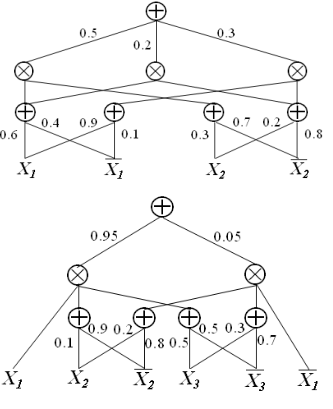
\includegraphics[scale=0.6]{Figures/SPN.png}
\end{figure}
The probability distribution of each leaf node is defined on a variable $V$, which can have finite states or be continuous. In the first case, the distribution is usually degenerate, i.e., there is a particular value $v^{*}$ of $V$ such that $P(v^{*}) = 1$ and $P(v) = 0$ otherwise (\textit{indicator}). When $V$ is continuous, the probability distribution can be Gaussian \cite{pmlr-v28-gens13}, \cite{pmlr-v32-rooshenas14}, piecewise polynomial \cite{DBLP:journals/corr/abs-1710-03297}, etc. (SPNs can be further generalized by allowing each terminal node to represent a multivariate probability density - for example, a multivariate Gaussian \cite{DBLP:journals/corr/DesanaS16} or a Chow-Liu tree \cite{10.1007/978-3-319-23525-7_21}).

An SPN can be built bottom-up beginning with sub-SPNs of one node and joining them with sum and product nodes. All the definitions of SPNs can be established recursively, first for one-node SPNs, and then for sum and product nodes. Similarly, all the properties of SPNs can be proved by structural induction.

If the probability distribution of a leaf node is defined on $V$, its \textit{scope} is the set ${V}$. If $n_i$ is a sum or a product node, its \textit{scope} is the union of the scopes of its children. Let $\mathsf{ch(n)}$ denote the set of children of a node. The \textit{scope} of an SPN, denoted by $\phi(\mathsf{S})$, is the scope of its root, $\phi(\mathsf{n_r})$. The variables in the scope of an SPN are sometimes called \textit{model variables} (in contrast with \textit{latent variables}.

Without going into detail, SPNs parameter learning consists in finding the optimal parameters for an SPN given its graph and a dataset. In generative learning the most common optimality criterion is to maximize the likelihood of the parameters of the model given a dataset, while in discriminative learning the goal is to maximize the conditional likelihood for each value of a variable C, called the class.

SPN allow to perform \textit{probabilistic inference}, i.e. deriving the probability of one or more RVs taking a specific value or a set of values. Exact and efficient probabilistic inference is important when we want to reason and quickly take complex decisions in presence of uncertainty in real-world scenarios. Probabilistic inference can be organized in classes of queries. Informally, a class of queries comprises of all the queries that share the same "structure", and hence present the same computational challenges. More formally, a class of queries is a collection of functions that operate on probability distributions and that can be characterized by the mean of their inputs, outputs and/or by the operations their computation involves \cite{ProbCirc20}. Here, we report several classes of queries which are used to compare and classify probabilistc models. 

\begin{definition}{\textbf{(Complete evidence queries - $\mathsf{EVI}$)}}
\label{def:evi}
The class of complete evidence queries $\boldsymbol{\mathcal{Q}}_{\mathsf{EVI}}$ is the set of queries that compute the probability $p_{\mathbf{X}}(\mathbf{x})$ for any complete evidence $\mathbf{x} \in \mathsf{val}(\mathbf{X})$.
\end{definition}

\begin{definition}{\textbf{(Marginal queries - $\mathsf{MAR}$)}}
\label{def:mar}
The class of marginal queries $\boldsymbol{\mathcal{Q}}_{\mathsf{MAR}}$ is the set of queries that compute the probability $p_{\mathbf{X}}(\mathbf{y})$ for any partial evidence $\mathbf{y} \in \mathsf{val}(\mathbf{Y})$, where $\mathbf{Y} \subseteq \mathbf{X}$.
\end{definition}

\begin{definition}{\textbf{(Conditional queries - $\mathsf{CON}$)}}
\label{def:con}
The class of conditional queries $\boldsymbol{\mathcal{Q}}_{\mathsf{CON}}$ is the set of queries that compute the probability $p_{\mathbf{X}}(\mathbf{y} | \mathbf{z})$ for any $\mathbf{y} \in \mathsf{val}(\mathbf{Y})$ and $\mathbf{z} \in \mathsf{val}(\mathbf{Z})$ , where $\mathbf{Y} \cup \mathbf{Z} = \mathbf{X}$ and $\mathbf{Y} \cap \mathbf{Z} = \varnothing$.
\end{definition}
It should be noticed that is possible to easily define the class $\boldsymbol{\mathcal{Q}}_{\mathsf{CON}}$ in terms of $\boldsymbol{\mathcal{Q}}_{\mathsf{EVI}}$ and $\boldsymbol{\mathcal{Q}}_{\mathsf{MAR}}$ by noting that any conditional query $p(x|y)$ can be rewritten as $p(x,y) / p(y)$.

\begin{definition}{\textbf{(Maximum a posteriori queries - $\mathsf{MAP}$)}}
\label{def:map}
The class of maximum a posteriori queries $\boldsymbol{\mathcal{Q}}_{\mathsf{MAP}}$ is the set of queries that compute:
\begin{align*}
	\argmax_{z \in \mathsf{val}(\mathbf{Z})} p_{\mathbf{X}}(\mathbf{z}|\mathbf{y}) = \argmax_{z \in \mathsf{val}(\mathbf{Z})} p_{\mathbf{X}}(\mathbf{z},\mathbf{y})
\end{align*}
where $\mathbf{Y} \cup \mathbf{Z} = \mathbf{X}$ and $\mathbf{Y} \cap \mathbf{Z} = \varnothing$.
\end{definition}
More classes of queries can be defined by "combining" the previous ones.
This is the case for marginal $\mathsf{MAP}$ queries ($\boldsymbol{\mathcal{Q}}_{\mathsf{MMAP}}$), involving marginalization over one subset of RVs and maximization over another one.

Recently, new advanced probabilistic queries have been introduced in literature.
These  include  computing  the  probability  of  an  event  described  as  a  complex logical sentence (e.g., involving disjunctions) \cite{choi2015tractable}; computing expectations of probabilistic predictive models \cite{khosravi2019tractable} and information theoretic quantities of a distribution such as its entropy or the Kullback-Leibler divergence between distributions \cite{liang2017towards}.
In the following, we will refer to the class of advanced queries as $\boldsymbol{\mathcal{Q}}_{\mathsf{ADV}}$.

Several well-known structural properties allow us to categorize PCs w.r.t. the classes of queries they make tractable.
% In fact, to make a class of queries $\boldsymbol{\mathcal{Q}}$ tractable for a PC, this has to satisfy specific structural constraints.
In the following, we first report the definition of tractability and then such structural properties indicating the class of queries they make tractable if satisfied.

\begin{definition}{\textbf{(Tractability)}}
A class of queries $\boldsymbol{\mathcal{Q}}$ is tractable on a family of probabilistic models $\mathcal{M}$ iff any query $q \in \boldsymbol{\mathcal{Q}}$ on a model $\mathsf{m} \in \mathcal{M}$ can be computed in time $O(poly(|\mathsf{m}|))$, where $|\mathsf{m}|$ is the size of the model.
\end{definition}

\begin{definition}{\textbf{(Smoothness, \textit{aka} Completeness)}}
A probabilistic circuit is \textbf{\textit{smooth}} if for each sum node $\mathsf{S}$ it hols that:
\begin{equation}\label{eq:completeness}
\forall \mathsf{C_1},\mathsf{C_2} \in \mathsf{ch}(\mathsf{S}) : \phi(\mathsf{C_1}) = \phi(\mathsf{C_2})
\end{equation}
\end{definition}

\begin{definition}{\textbf{(Decomposability)}}
A probabilistic circuit is \textbf{\textit{decomposable}} if for each product node $\mathsf{P}$ it hols that:
\begin{equation}\label{eq:decomposability}
\forall \mathsf{C_1},\mathsf{C_2} \in \mathsf{ch}(\mathsf{P}), \mathsf{C_1} \neq \mathsf{C_2} : \phi(\mathsf{C_1}) \cap \phi(\mathsf{C_2}) = \varnothing
\end{equation}
\end{definition}

\noindent  To allow for efficient inference, PCs should satify the structural constraints \ref{eq:completeness} and \ref{eq:decomposability}.
In that way, all nodes in an PC recursively define a distribution over their respective scopes: the leaves are distributions by definition, sum nodes are mixtures of their child distributions, and products are factorized distributions, assuming (conditional) independence among the scopes of their children.
Smooth and decomposable PCs enable the tractable computation of any marginal query ($\mathsf{MAR}$ inference) and thus also of any conditional one ($\mathsf{CON}$ inference).

\begin{definition}{\textbf{(Determinism, \textit{aka} Selectivity)}}
A probabilistic circuit is \textbf{\textit{deterministic}} if for every sum node $\mathsf{S}$ and input $\mathbf{x}$, at most one of the children of $\mathsf{S}$ has a non-zero output, i.e. children distribuions have disjoint support.
\end{definition}

\noindent A deterministic sum defines a mixture model whose components have disjoint support, enabling tractable $\mathsf{MAP}$ queries.
A decomposable and deterministic PC ensures $\mathsf{MAP}$ tractable queries.

\begin{definition}{\textbf{(Vtree)}} A vtree $\mathcal{V}$ of a set of variables $\mathbf{X}$ is an n-ary tree where every leaf node uniquely denotes a RV and every internal node denotes the set of RVs equal to the union of the RVs denoted by its children, so that the root of $\mathcal{V}$ denotes $\mathbf{X}$.
In other words, a vtree $\mathcal{V}$ over $\mathbf{X}$ represent a hierarchical decomposition of the RVs in $\mathbf{X}$.
\end{definition}

\begin{definition}{\textbf{(Structured-Decomposability)}} A probabilistic circuit is normalized for a vtree $\mathcal{V}$ if the scope of every product node $\mathsf{P}$ decomposes over its children as its corresponding node, i.e. the one denoting the scope of $\mathsf{P}$.
A circuit is \textbf{\textit{structured decomposable}} if it is normalized for some vtree.
The circuit is then decomposable.
\end{definition}

\noindent A trivial test for structured decomposability is ensuring that for every possible pair of product nodes $\langle \mathsf{P_1}, \mathsf{P_2} \rangle$ in a PC, either $\phi(\mathsf{P_1}) \subseteq \phi(\mathsf{P_2})$ or $\phi(\mathsf{P_2}) \subseteq \phi(\mathsf{P_1})$.
By enforcing structured decomposability, several classes of advanced probabilistic queries, which we denoted as $\boldsymbol{\mathcal{Q}}_{\mathsf{ADV}}$, become computable exactly and efficiently. 

\subsection{Random And Tensorized SPNs (RAT-SPNs)}
\label{rat-spn}
Sum-product networks are an excellent architecture that allows to efficiently evaluate likelihoods, as well arbitrary marginalization and conditioning tasks. Nevertheless, SPNs have not been fully explored as serious deep learning models, likely due to their special structural requirements, which complicate learning. Peharz et al. \cite{DBLP:journals/corr/abs-1806-01910} make a drastic simplification and use random SPN structures which are trained in a "classical deep learning manner", i.e. employing automatic differentiation, SGD and GPU support. The resulting models, called \textit{Random And Tensorized SPNs} (RAT-SPNs), yeld prediction results comparable to deep neural networks, while stille being interpretable as generative model and maintaining well-calibrated uncertainties. This property makes them highly robust under missing input features and enables them to naturally detect outliers and peculiar samples.

In order to construct Random And Tensorized SPNs, a region graph (\cite{poon2011sum}, \cite{pmlr-v28-gens13}, \cite{10.1007/978-3-642-40991-2_39}) is used as an abstract representation of the network structure. Given a set of RVSs \textbf{X}, a  \textit{region} \textbf{R} is defined as any non-empty sub-set of \textbf{X}. Given any region \textbf{R}, a  \textit{K-partition P} of \textbf{R} is a collection of \textit{K} non-empty, non overlapping subsets $\mathbf{R}_1$,...,$\mathbf{R}_K$ of \textbf{R}, whose union is again \textbf{R}. In RAT-SPNs only 2-partitions are considered, so that all product nodes in resulting SPNs have exactly two children. This assumption, frequently made in SPN literature, simplifies SPN design and seems not to impair performance.

A  \textit{region graph R} over \textbf{X} is a DAG whose nodes are regions and partitions such that:
\begin{enumerate}[I.]
  \item \textbf{X} is a region in R and has no parents (root region);
  \item all other regions have at least one parent;
  \item all children of regions are partitions an all children of partitions are regions (i.e., \textit{R} is bipartitive);
  \item if \textit{P} is a child of \textbf{R}, then $\bigcup_{\mathbf{R^\ast}\in\mathit{P}}\mathbf{R^\ast} = \mathbf{R}$;
  \item if \textbf{R} is a child of \textit{P}, then \textbf{R} $\in$ \textit{P}.
\end{enumerate}
From this definition it follows that a region graph dictates a hierarchical partition of the overall scope \textbf{X}. We denote regions which have no child partitions as \textit{leaf regions}.

Given a region graph, a corresponding smooth (complete) and decomposable SPN can be constructed, as illustrated in Algorithm \ref{alg:rg-to-spn}. Random region graphs are constructed using the simple procedure depicted in Algorithm \ref{alg:random-region-graph}. The root region is randomly divided into two sub-regions of equal size and . This recursive splitting mechanism is repeated R times. Figure \ref{fig:rat-spn} shows an example SPN with \textit{C} = 3, \textit{S} = 2 and \textit{I} = 3, following Algorithm \ref{alg:random-region-graph} and subsequentially Algorithm \ref{alg:rg-to-spn}. Note that this construction scheme yields SPNs where input distributions, sums, and products can be naturally organized in alternating layers. Similar to classical multilayer perceptrons (MLPs), each layer takes inputs from its directly preceding layer only. Unlike MLPs, however, layers in RAT-SPNs are connected block-wise sparsely in a random fashion. Thus, layers in MLPs and RAT-SPNs are hardly comparable; however, we suggest to understand each pair of sum and product layer to be roughly corresponding to one layer in an MLP: sum layers play the role of (block-wise sparse) matrix multiplication and product layers as non-linearities (or, more precisely, bilinearities of their inputs). The input layer, containing the SPN’s leaf distributions, can be interpreted as a non-linear feature extractors.

\begin{algorithm}[H]
\caption{Construct SPN from Region Graph}
\label{alg:rg-to-spn}
\small
\begin{algorithmic}[1]
\Input{\textit{R}: region graph; \textit{C}: number of classes; \textit{S}: number of sum nodes in regions, which are neither leaf nor root regions; \textit{I}: number of input distributions per leaf region.}
\Output{A smooth and decomposable SPN deriving from region graph \textit{R}}
\State Make empty SPN
\ForEach{$\mathbf{R} \in \mathit{R}$}
	\If {$\mathbf{R}$ is a leaf region}
		\State Equip $\mathbf{R}$ with $\mathit{I}$ distribution nodes
	\ElsIf {$\mathbf{R}$ is the root region}
		\State Equip $\mathbf{R}$ with $\mathit{C}$ sum nodes
	\Else
		\State Equip $\mathbf{R}$ with $\mathit{S}$ sum nodes 
	\EndIf
\EndFor
\ForEach{$\mathit{P} = \{\mathbf{R}_1,\mathbf{R}_2\} \in \mathit{R}$}
	\State Let $\mathbf{N_R}$ be the nodes for region $\mathbf{R}$
	\ForEach{$N_1 \in \mathbf{N_{R_1}}, N_2 \in \mathbf{N_{R_2}}$}
		\State Introduce product $P = N_1 \cdot N_2$
		\State Let P be a child for each $N \in \mathbf{N_{R_1 u \cup R_2}}$
	\EndFor
\EndFor
\State \Return SPN
\end{algorithmic}
\end{algorithm}

\begin{algorithm}[H]
\caption{Random Region Graph}
\label{alg:random-region-graph}
\small
\begin{algorithmic}[1]
\Input{\textbf{X}: set of RVs; \textit{D}: depth; \textit{R}: number of recursive splits.}
\Output{A random region graph}
\State Create an empty region graph $\mathfrak{R}$
\State Insert $\mathbf{X}$ in $\mathfrak{R}$
\ForEach{$r = 1 ... \mathit{R}$}
	\State SPLIT($\mathit{R},\mathfrak{R},\mathit{D}$)
\EndFor
\end{algorithmic}

\begin{algorithmic}[1]
\Procedure {SPLIT}{$\mathit{R},\mathbf{R},\mathit{D}$}
	\State Draw balanced partition $\mathit{P} = \{ \mathbf{R}_1,\mathbf{R}_2 \}$ of $\mathbf{R}$
	\State Insert $\mathbf{R}_1,\mathbf{R}_2$ in $\mathit{R}$
	\State Insert $\mathit{P}$ in $\mathit{R}$
	\If {$\mathit{D} > 1$}
		\If {$|\mathbf{R}_1| > 1$}
			\State SPLIT$(\mathit{R},\mathbf{R}_1,\mathit{D}-1)$
		\EndIf
		\If {$|\mathbf{R}_2| > 1$}
			\State SPLIT$(\mathit{R},\mathbf{R}_2,\mathit{D}-1)$
		\EndIf
	\EndIf
\EndProcedure
\end{algorithmic}
\end{algorithm}

\begin{figure}[H]
\caption{Example RAT-SPN over 7 RVs \{$\mathit{X}_1$,...,$\mathit{X}_7$\}, using parameters \textit{C} = 3, \textit{D} = 2, \textit{R} = 2, \textit{S} = 2 and \textit{I} = 2 in Algorithm \ref{alg:random-region-graph} and Algorithm \ref{alg:rg-to-spn}.}
\label{fig:rat-spn}
\centering
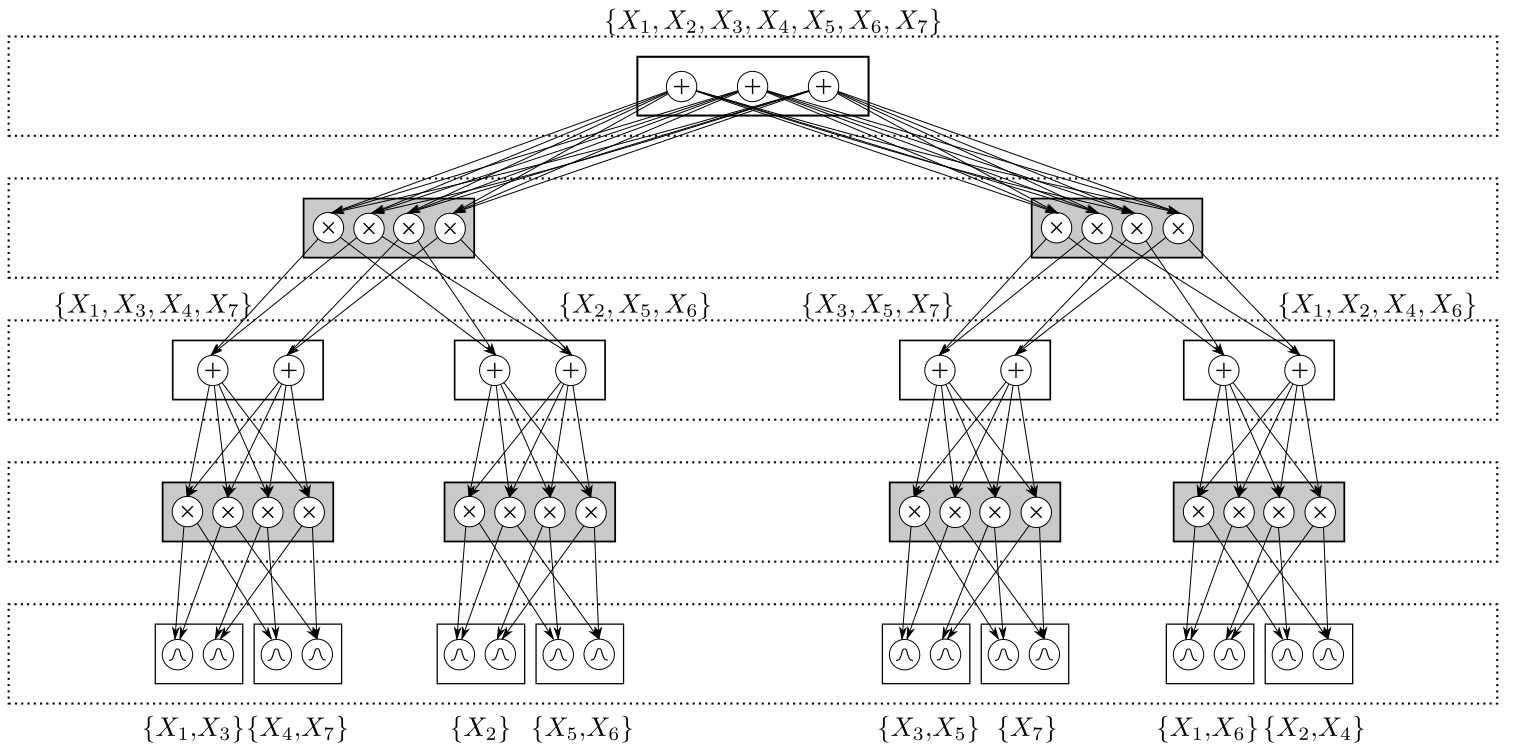
\includegraphics[scale=0.265]{Figures/RAT-SPN.png}
\end{figure}
As mentioned above, RAT-SPNs are trained in a "classical deep learning manner", i.e. employing automatic differentiation, SGD and GPU support. More specifically, let $\mathit{X} = \{(\mathbf{x}_1,\mathit{y}_1),...,(\mathbf{x}_N,\mathit{y}_N)$ be a training set of input $\mathbf{x}_n$ and class labels $\mathbf{y}_n$. Furthermore, let $\mathit{S}_C$ be the $c^{th}$ output of the RAT-SPN and $\mathbf{w}$ all SPN parameters. RAT-SPNs training is performed by minimizing the objective

\begin{equation}\label{objective}
	O(\mathbf{w}) = \lambda \mathbf{CE}(\mathbf{w}) + (1-\lambda)n\mathbf{LL}(\mathbf{w})
\end{equation}

where $\mathbf{CE}(\mathbf{w})$ is the cross-entropy

\begin{equation}\label{cross-entropy}
	\mathbf{CE}(\mathbf{w}) = -\frac{1}{\mathit{N}}\sum_{n} log\frac{\mathit{S}_{\mathit{y_n}}(\mathbf{x}_n)}{\sum_{\mathit{y'}}\mathit{S}_{\mathit{y'}}(\mathbf{x}_n)}
\end{equation}

and n$\mathbf{LL}(\mathbf{w})$ is the normalized negative log-likelihood

\begin{equation}\label{nll}
	n\mathbf{LL}(\mathbf{w}) = -\frac{1}{\mathit{N}|\mathbf{X}|}\sum_{n} log\mathit{S}_{\mathit{y_n}}.
\end{equation}
When setting $\lambda = 1$, purely cross-entropy is optimized (discriminative setting), while for $\lambda = 0$ maximum likelihood training is performed (generative setting). For $0 < \lambda < 1$, we have a continuum of hybrid objectives, trading off the generative and dsicriminative character of the model.

The size of RAT-SPN can be easily controlled via the structural parameters \textit{D}, \textit{R}, \textit{S} and \textit{I}. RAT-SPNs with many parameters, however, tend to overfit just like regular neural networks, which requires regularization. One of the classical techniques that boosted deep learning models is the well-known \textit{dropout} heuristic \cite{srivastava2014dropout}, setting inputs and/or hidden units to zero with a certain probability \textit{p}, and rescaling the remaining units by $\frac{1}{\mathit{p}}$. In RAT-SPNs two types of dropout are exploited:

\begin{enumerate}[I.]
  \item \textit{Dropout at inputs.} It essentially consists in marking input features as missing at random;
  \item \textit{Dropout at sums.} As discussed in [\cite{poon2011sum}, \cite{DBLP:journals/corr/ZhaoMP15}, \cite{DBLP:journals/corr/PeharzGPD16}], sum nodes in SPNs can be interpreted as marginalized latent variables, akin to the latent variable interpretation in mixture models. In RAT-SPNs a whole region can be interpreted as a single latent variable, and the weights of each sum node in this region as the conditional distribution of this variable. While the latent variables are not observed, the idea is to employ a simple probabilistic version of dropout, by introducing artificial observations for them. For example, if the sum nodes in a particular region have \textit{K} children (i.e. the corresponding variable \textit{Z} has \textit{K} states), then the artificial information that \textit{Z} assumes a state in some subset of $\{1,...,\mathit{K}\}$ can be introduced. By doing this for each latent variable in the network, the results essentially consists in selecting a small sub-structure of the whole SPN to explain the data. 
\end{enumerate}

\section{Abduction}
A central theme in the study of human reasoning is the construction of explanations that give us an understanding of the world we live in. Broadly speaking, abduction is a reasoning process invoked to explain a puzzling observation. A typical example is a practical competence like medical diagnosis. When a doctor observes a symptom in a patient, he hypothesizes about its possible causes, based on his knowledge of the causal relations between diseases and symptoms. This is a practical setting. Abduction also occurs in more theoretical scientific contexts. For instance, it has been claimed \cite{Peirce1932} that when Kepler discovered that Mars had an elliptical orbit, his reasoning was abductive.

Charles Sanders Peirce (1839-1914), the founder of American pragmatism was the first philosopher to give a logical form to abduction. In his early theory Peirce proposed three modes of reasoning: deduction, induction and abduction, each oh which corresponds to a syllogistic form, illustrated by the following, often quoted example \cite{Peirce1932}:
\vspace{1\baselineskip}

\textit{DEDUCTION}

Rule - All the beans from this bag are white.

Case - These beans are from this bag.

Results - These beans are white.
\vspace{1\baselineskip}

\textit{INDUCTION}

Case - These beans are from this bag.

Result - These beans are white.

Rule - All the beans from this bag are white.
\vspace{1\baselineskip}

\textit{ABDUCTION}

Rule - All the beans from this bag are white.

Results - These beans are white.

Case - These beans are from this bag.
\vspace{1\baselineskip}

Of these, deduction is the only reasoning which is completely certain, infering its 'Results' as a necessary conclusion. Induction produces a 'Rule' validated only in the 'long run' \cite{Peirce1932}, and abduction merely suggests that something may be 'the Case' \cite{Peirce1932}. The abduction is, according to Peirce, the only reasoning form that can increase our knowledge, i.e. suggest new ideas, gueess, predict. Actually, all three inference mechanisms described above allow to increase our knowledge, even if in different order and measure, but only abduction is entirely aimed at this increase. It is also true that abduction is the most subjected to error. As with induction, abduction does not contain in itself its logic validity and it has to be empirically validated; it will never be possible to have an absolute validation, but only a probabilistic one.

In the context of formal logic, abduction is often defined as follows:

\begin{definition}{\textbf{(Abduction)}}
\label{def:abduction}
Given a logical theory $\mathit{T}$ representing the expert knowledge and a formula $\mathit{Q}$ representing an observation on the problem domain, abductive inference searches for an explanation formula $\varepsilon$ such that:
\begin{itemize}
  \item $\varepsilon$ is satisfiable\footnote{If $\varepsilon$ contains free variables, $\exists(\varepsilon)$ should be satisfiable w.r.t. $\mathit{T}$.} w.r.t. T and
  \item it holds that\footnote{Or, more general, if $\mathit{Q}$ and $\varepsilon$ contain free variables: $\mathit{T} \models \forall(\varepsilon \rightarrow \mathit{Q}) $} $\mathit{T} \models \varepsilon \rightarrow \mathit{Q}$.
\end{itemize}
\end{definition}
In general, $\varepsilon$ will be subjected to further restrictions such as the aforementioned minimality criteria and criteria restricting the form of the explanation formula (e.g. by restricting the predicates that may appear in it). This view defines an abductive explanation of an observation as a formula which \textit{logically entails} the observation. However, some have argued, sometimes with good reasons, that it is more natural to view an explanation as a \textit{cause} for the observation. A well-known example is as follows: the disease paresis is caused bya latent untreated form of syphilis. The probability that latent untreated syphilis leads to paresis is only 25\%. Note that in this context, the direction of entailment and causalityare opposite: syphilis is the cause of paresis but does not entail it, while paresis entails syphilis but does not cause it. Yet a doctor can \textit{explain} paresis by the hypothesis of syphilis while paresis cannot account for an \textit{explanation}s for syphilis.

In practice, examples where causation and entailment do not correspond are rare. It turns out that in many applications of abduction in AI, the theory T describes explicit \textit{causality information}. This is notably the case in model-based diagnosis and in temporal reasoning, where theories describe effects of actions. By restricting the explanation formulas to the predicates describing primitive causes in the domain, an explanation formula which entails an observation gives a cause for the observation. Hence, for this class of theories, the logical entailment view implements the causality view on abductive inference.

In the context of logic programming, the study of abductive inference started at the end of the eighties as an outcome of different attempts to use logic programming for solving AI-problems. Facing the limitations of standard logic programming for solving these problems, different researchers proposed to extend logic programming with abduction. Eshghi \cite{Eshghi198801562579} introduced abduction in logic programming in order to solve planning problems in the Event Calculus \cite{Kowalski1989}. In this approach, abduction solves a planning goal by explaining it byan ordered sets of events -a plan- that entails the planning goal. This approach was further explored byShanahan \cite{Shanahan198901}, Missiaen et al. \cite{Eshghi198801562579},\cite{10.1093/logcom/5.5.579}, Denecker \cite{Denecker200112}, Jung \cite{SHANAHAN2000207} and recently in \cite{Kakas1998ACLPAC},\cite{KAKAS2000129}. In parallel to these studies of abduction as an inferential method, Eshghi and Kowalski \cite{Eshghi198801234235} and later Kakas and Mancarella in \cite{Kakas199001},\cite{Kakas1990OnTR} and Dung in \cite{Dung1991NegationsAH}, used abduction as a semantical device to describe the non-monotonic semantics of Logic Programming (in a wayanalogous to Poole in \cite{POOLE198827}). In \cite{Denecker2001125},\cite{10.1007/3-540-59487-6_2}, abductive logic programming was investigated from a knowledge representation point of view and its suitabilityfor representing and reasoning on incomplete information and definitional and assertional knowledge was shown. For these reasons, Abductive Logic Programming1 (ALP) \cite{10.1093/logcom/2.6.719},\cite{Kakas98therole} was recognized as a promising computational paradigm that could resolve many limitations of logic programming with respect to higher level knowledge representation and reasoning tasks. ALP has manifested itself as a framework for declarative problem solving suitable for a broad collection of problems.

\section{Classification}
\label{classification}
\textit{Classification} is a type of supervised learning that consists in building a classifier from a set of examples labeled by their classes or precedents (learning step) and then predicting the class of new examples by using the generated classifiers (classification step). More formally, let:

\begin{itemize}
  \item $\mathit{X}$ be the instance space (whose elements correspond to the observations);
  \item $\mathit{C}$ be a non-empty finite set (whose elements correspond to the classes/labels);
  \item $\mathit{c}: \mathit{X} \rightarrow \mathit{C}$ be the classification function to be learned;
  \item $\mathit{H}$ be the hypothesis space;
  \item $\mathit{h} \in \mathit{H}$ such that $h: \mathit{X} \rightarrow \mathit{C}$.
\end{itemize}
Given a sequence of training examples $\{(\mathbf{x}_1,\mathit{c}_1),...,(\mathbf{x}_n,\mathit{c}_n)\}$, where  $\mathbf{x}_i \in \mathit{X}$, $\mathit{c}_i \in \mathit{C}$ and $\mathit{c}_i = \mathit{c}(\mathbf{x}_i)$, the goal is to find $\mathit{h}$ such that $\mathit{h}(\mathbf{x}_i) = \mathit{c}(\mathbf{x}_i)$ $\forall \mathbf{x}_i \in \mathit{X}$.

In this thesis work, we are interested in a slightly different classification task, in which the known information about training examples is not directly their associated class but an aggregate information deriving from it. More formally, this task differs from the one described above in the following respects:

\begin{itemize}
  \item let $\mathit{f}: \mathit{C} \times ... \times \mathit{C} \rightarrow \mathit{F}$ be an aggregate non-injective function with arity $m$, where $\mathit{F}$ is a non-empty finite set;
  \item training examples form is $\{((\mathbf{x}_1,...,\mathbf{x}_m),\mathit{f}_1),...,((\mathbf{x}_{n-m+1},...,\mathbf{x}_n),\mathit{f}_{\frac{n}{m}})\}$, 
  where $\mathbf{x}_i \in \mathit{X}$, $\mathit{f}_i \in \mathit{F}$ and 
\begin{equation}\
	\mathit{f}_i = \mathit{f}(\mathit{c}_{m(i-1)+1},...,\mathit{c}_{m(i-1)+1+m}) = \mathit{f}(\mathit{c(\mathbf{x}_{m(i-1)+1})},...,\mathit{c(\mathbf{x}_{m(i-1)+1+m})}).
\end{equation}
\end{itemize}
Basically, training examples are grouped into tuples with cardinality $m$, on whose corresponding labels a function $\mathit{f}$ is applied. Note that:

\begin{itemize}
  \item the classifier knows how to compute $\mathit{f}$ (and this information will be encapsulated in the knowledge domain of the symbolic module); 
  \item if $\mathit{f}$ was injective, such classification task just would come back to the "standard" one, since the model would be able to deterministically derive the correct classes from the aggregate information.
\end{itemize} 
\chapter{Model}
\label{Chapter3}
This chapter aims to totally describe the proposed model. Before going into the description details, Section \ref{challenge} tries to frame the difficulties that the model has to deal with, in trying to solve a classification task of the one described in Section \ref{classification}. These observations aim to provide a preliminary justification and comprehension of the reasons behind specific choices.

\section{What is the challenge?}
\label{challenge}
\begin{table}[H]
  \centering
  \caption{Performance of some configurations of a simple Neural-Symbolic model. All accuracy values are in percentage and approximated to the second digit after the decimal place.}
  \label{tab:simple-model}
  \scriptsize
  \begin{tabular}{ccccccrr}
    \toprule
    depth		& distributions 			& splits 		& sums 				& dropout input 		& dropout sums 			& valid acc 			& test acc\\
    \midrule
    1			& 10						& 9 			& 10 				& 0.5 					& 0.75 					& 95.03 				& 94.88\\
	1			& 10						& 9 			& 10 				& 0.5 					& 1 					& 27.55 				& 26.78\\
	1			& 10						& 9 			& 10 				& 0.75 					& 1 					& 97 .01				& 96.11\\
	\textbf{1}	& \textbf{10}				& \textbf{9} 	& \textbf{10} 		& \textbf{0.25} 		& \textbf{0.25} 		& \textbf{6.12} 		& \textbf{5.74}\\
	1			& 10						& 9 			& 10 				& 0.50 					& 0.25 					& 94.51 				& 94.65\\
	1			& 10						& 9 			& 10 				& 0.25 					& 0.5 					& 94.48 				& 94.08\\
	1			& 33						& 40 			& 10 				& 0.25 					& 0.5 					& 92.92 				& 92.75\\
	1			& 33						& 40 			& 10 				& 0.5 					& 0.25 					& 59.13 				& 58.93\\
	1			& 33						& 40 			& 10 				& 0.75 					& 0.25 					& 84.22 				& 84.75\\
	1			& 33						& 40 			& 10 				& 0.25 					& 1 					& 19.83 				& 19.96\\
    1			& 33						& 40 			& 10 				& 0.5 					& 1 					& 96.27 				& 96.24\\
	1			& 33						& 40 			& 10 				& 0.5 					& 0.5 					& 96.53 				& 96.16\\
    \bottomrule
  \end{tabular}
\end{table}
Table \ref{tab:simple-model} shows the performance of some configurations (for brevity) of a very simple Neural-Symbolic model, whose subsymbolic module training is based on the most probable abduction among the ones suggested by the symbolic module; the task consists in learning to classify digits from 0 to 9, knowing the sum of $n$ pairs of them. For the moment, further details about the classification task and the model under consideration are intentionally omitted, in order to focus the attention on the findings. Looking at the results, a significant variance in terms of accuracy is evident among the tested configurations. In order to investigate this anomalous behaviour and to understand if such a variance depends on the specific configuration (i.e. on the the sub-symbolic hyperparameters) or not, the configuration highlighted in bold in Table \ref{tab:simple-model} has been runned multiple times.

\begin{table}[H]
  \caption{Multiple runs of configuration higlighted in bold in Table \ref{tab:simple-model}. Reported values refer to accuracy computed on validation set (in percentage).}
  \label{tab:multiple-run}
  \centering
  \renewcommand{\arraystretch}{0.8}
  \begin{tabular}{cccc}  
    %\toprule
						& \textbf{run 1} & \textbf{run 2} & \textbf{run 3} \\
	\hline
	\textbf{epoch 0}	& 14.98 			& 47.21 		& 33.91  \\
	\hline
	\textbf{epoch 30}	& 11.65 			& 70.85 		& 52.15  \\
	\hline
	\textbf{epoch 50}	& 10.32 			& 90.12 		& 78.92  \\
	\hline
	\textbf{epoch 100} 	& 12.79				& 93.22 		& 88.34  \\
	\bottomrule
	\end{tabular}
\end{table}
Results of Table \ref{tab:multiple-run} clearly show that the variance in the model performance does not depend on the considered combination of hyperparameters, since multiple runs of the same configuration bring to very different values in terms of accuracy. With the aim of furtherly investigate this attitude, Tables \ref{tab:confusion-matrix-1}, \ref{tab:confusion-matrix-2} and \ref{tab:confusion-matrix-3} show the confusion matrices of the first epoch of such runs, calculated taking into account the real labels of the considered digits and the labels selected by the sub-symbolic module among the ones suggested by symbolic one. In particular, since each value has been obtained dividing the observed frequency by the correspondent row sum, the element in position $(i,j)$ indicates the ratio with which the $i-th$ digit has been labeled as the $j-th$ one by the model (the reverse observation can NOT be done). These matrices point out that the strong variance in terms of accuracy lies in the variability with whom the examples are labelled on the basis of the symbolic module abductions and the subsymbolic module probabilities. Since the initialization of the subsymbolic module is random and since the most probable abduction is chosen according to the probability computed by the SPN, selected abductions to train the model are random likewise. Therefore, since the model has no way to understand if it is going well or not, the first taken direction significantly influences all the training procedure. Essentially, the model goodness depends on chance: only if the first abduced labels are (by chance) correct, the model performance are quite good. It is clear that this behaviour can't be considered as a real learning. Furthermore, the more the task becomes difficult (in terms of the number of possible abductions), the more the chance of randomly abducing the correct labels decreases. 

The considerations made up to now emphasise that, since the abduction is not a reasoning process that returns always true facts and especially because the initialization of the subsymbolic model is randomic, we need to try to force the model not to learn from abductions it is not sufficently sure of, trying to guide somehow it towards the real most probable ones. All the choices explained in the following section are oriented in this perspective.

\begin{table}[H]
  \caption{Confusion matrix between real labels (row) and abduced labels (column) for run 1 of Table \ref{tab:multiple-run}. Each reported value has been obtained dividing the observed frequency by the correspondent row sum and approximated to the second digit after the decimal place. Accuracy on validation set: 14.98\%}
  \label{tab:confusion-matrix-1}
  \centering
  \begin{tabular}{ccccccccccc}  
    %\toprule
						& \textbf{0} & \textbf{1} & \textbf{2} & \textbf{3} & \textbf{4} & \textbf{5} & \textbf{6} & \textbf{7} & \textbf{8} & \textbf{9}\\
	\hline
	\textbf{0}			& \textbf{0.27} & 0.17 & 0.27 & 0.06 & 0.06 & 0.04 & 0.03 & 0.09 & 0.00 & 0.00  \\
	\hline
	\textbf{1}			& 0.14 & \textbf{0.21} & 0.17 & 0.08 & 0.14 & 0.25 & 0.00 & 0.00 & 0.00 & 0.00  \\
	\hline
	\textbf{2}			& 0.14 & 0.11 & \textbf{0.26} & 0.09 & 0.12 & 0.13 & 0.03 & 0.06 & 0.05 & 0.02  \\
	\hline
	\textbf{3} 			& 0.06 & 0.09 & 0.23 & \textbf{0.09} & 0.09 & 0.25 & 0.06 & 0.06 & 0.05 & 0.02  \\
	\hline
	\textbf{4} 			& 0.04 & 0.06 & 0.17 & 0.09 & \textbf{0.09} & 0.31 & 0.12 & 0.06 & 0.05 & 0.02  \\
	\hline
	\textbf{5} 			& 0.06 & 0.06 & 0.08 & 0.07 & 0.13 & \textbf{0.26} & 0.11 & 0.09 & 0.09 & 0.05  \\
	\hline
	\textbf{6} 			& 0.03 & 0.02 & 0.10 & 0.04 & 0.16 & 0.20 & \textbf{0.16} & 0.19 & 0.06 & 0.05  \\
	\hline
	\textbf{7} 			& 0.02 & 0.01 & 0.05 & 0.04 & 0.08 & 0.27 & 0.16 & \textbf{0.10} & 0.16 & 0.11  \\
	\hline
	\textbf{8} 			& 0.00 & 0.03 & 0.05 & 0.02 & 0.09 & 0.15 & 0.13 & 0.10 & \textbf{0.31} & 0.11  \\
	\hline
	\textbf{9} 			& 0.00 & 0.00 & 0.06 & 0.02 & 0.03 & 0.20 & 0.13 & 0.09 & 0.22 & \textbf{0.25}  \\
	\bottomrule
	\end{tabular}
\end{table}

\begin{table}[H]
  \caption{Confusion matrix between real labels (row) and abduced labels (column) for run 2 of Table \ref{tab:multiple-run}. Each reported value has been obtained dividing the observed frequency by the correspondent row sum and approximated to the second digit after the decimal place. Accuracy on validation set: 47.21\%}
  \label{tab:confusion-matrix-2}
  \centering
  \begin{tabular}{ccccccccccc}  
    %\toprule
						& \textbf{0} & \textbf{1} & \textbf{2} & \textbf{3} & \textbf{4} & \textbf{5} & \textbf{6} & \textbf{7} & \textbf{8} & \textbf{9}\\
	\hline
	\textbf{0}			& \textbf{0.39} & 0.16 & 0.18 & 0.08 & 0.05 & 0.05 & 0.05 & 0.03 & 0.01 & 0.01  \\
	\hline
	\textbf{1}			& 0.09 & \textbf{0.41} & 0.11 & 0.18 & 0.06 & 0.01 & 0.01 & 0.11 & 0.02 & 0.00  \\
	\hline
	\textbf{2}			& 0.12 & 0.13 & \textbf{0.25} & 0.17 & 0.1  & 0.08 & 0.05 & 0.04 & 0.04 & 0.02  \\
	\hline
	\textbf{3} 			& 0.08 & 0.10 & 0.13 & \textbf{0.29} & 0.12 & 0.07 & 0.08 & 0.04 & 0.04 & 0.05  \\
	\hline
	\textbf{4} 			& 0.03 & 0.11 & 0.10 & 0.15 & \textbf{0.15} & 0.05 & 0.12 & 0.23 & 0.03 & 0.03  \\
	\hline
	\textbf{5} 			& 0.03 & 0.04 & 0.10 & 0.16 & 0.11 & \textbf{0.12} & 0.16 & 0.18 & 0.04 & 0.06  \\
	\hline
	\textbf{6} 			& 0.04 & 0.03 & 0.04 & 0.11 & 0.06 & 0.09 & \textbf{0.37} & 0.12 & 0.07 & 0.06  \\
	\hline
	\textbf{7} 			& 0.01 & 0.05 & 0.03 & 0.04 & 0.07 & 0.04 & 0.07 & \textbf{0.47} & 0.17 & 0.05  \\
	\hline
	\textbf{8} 			& 0.00 & 0.02 & 0.09 & 0.04 & 0.05 & 0.07 & 0.14 & 0.21 & \textbf{0.25} & 0.14  \\
	\hline
	\textbf{9} 			& 0.01 & 0.00 & 0.04 & 0.08 & 0.03 & 0.04 & 0.11 & 0.26 & 0.23 & \textbf{0.21}  \\
	\bottomrule
	\end{tabular}
\end{table}

\begin{table}[H]
  \caption{Confusion matrix between real labels (row) and abduced labels (column) for run 3 of Table \ref{tab:multiple-run}. Each reported value has been obtained dividing the observed frequency by the correspondent row sum and approximated to the second digit after the decimal place. Accuracy on validation set: 33.91\%}
  \label{tab:confusion-matrix-3}
  \centering
  \begin{tabular}{ccccccccccc}  
    %\toprule
						& \textbf{0} & \textbf{1} & \textbf{2} & \textbf{3} & \textbf{4} & \textbf{5} & \textbf{6} & \textbf{7} & \textbf{8} & \textbf{9}\\
	\hline
	\textbf{0}			& \textbf{0.39} & 0.12 & 0.22 & 0.08 & 0.03 & 0.03 & 0.10 & 0.01 & 0.00 & 0.02  \\
	\hline
	\textbf{1}			& 0.10 & \textbf{0.37} & 0.06 & 0.23 & 0.07 & 0.04 & 0.01 & 0.11 & 0.01 & 0.00  \\
	\hline
	\textbf{2}			& 0.14 & 0.07 & \textbf{0.33} & 0.14 & 0.08 & 0.04 & 0.10 & 0.03 & 0.04 & 0.03  \\
	\hline
	\textbf{3} 			& 0.06 & 0.12 & 0.06 & \textbf{0.41} & 0.08 & 0.10 & 0.03 & 0.05 & 0.04 & 0.05  \\
	\hline
	\textbf{4} 			& 0.07 & 0.07 & 0.09 & 0.14 & \textbf{0.19} & 0.10 & 0.11 & 0.19 & 0.03 & 0.03  \\
	\hline
	\textbf{5} 			& 0.04 & 0.04 & 0.07 & 0.18 & 0.07 & \textbf{0.22} & 0.08 & 0.17 & 0.05 & 0.08  \\
	\hline
	\textbf{6} 			& 0.07 & 0.01 & 0.04 & 0.09 & 0.05 & 0.05 & \textbf{0.44} & 0.11 & 0.07 & 0.07  \\
	\hline
	\textbf{7} 			& 0.01 & 0.07 & 0.02 & 0.05 & 0.06 & 0.06 & 0.04 & \textbf{0.54} & 0.07 & 0.08  \\
	\hline
	\textbf{8} 			& 0.01 & 0.02 & 0.08 & 0.06 & 0.05 & 0.10 & 0.11 & 0.25 & \textbf{0.17} & 0.15  \\
	\hline
	\textbf{9} 			& 0.02 & 0.00 & 0.02 & 0.09 & 0.02 & 0.07 & 0.08 & 0.34 & 0.13 & \textbf{0.23}  \\
	\bottomrule
	\end{tabular}
\end{table}

\section{Architecture and features}
\label{arch-and-feat}
Figure \ref{fig:architecture} shows the general architecture of the implemented model. Essentially:

\begin{itemize}
	\item the symbolic module, containing the domain knowledge, takes in input the aggregate information (elements of $\mathit{F}$ deriving from the application of function $\mathit{f}$, see Section \ref{classification}) related to the observations and returns all the possible abductions;
	\item the sub-symbolic module, which consists in a Random And Tensorized SPN (RAT-SPN), receives such explanations together with the observations and, on the basis of the most probable ones (i.e., abductions), performs the training process. Note that RAT-SPN is unuware about $\mathit{f}$, it just works on observations and labels abduced by symbolic module.
\end{itemize}
In the following, we describe in detail the implemented features (in the figure, red numbers from 1 to 4) that allow the final model to perform better than the one described in Section \ref{challenge}.

\begin{figure}[H]
\caption{Model architecture.}
\label{fig:architecture}
\centering
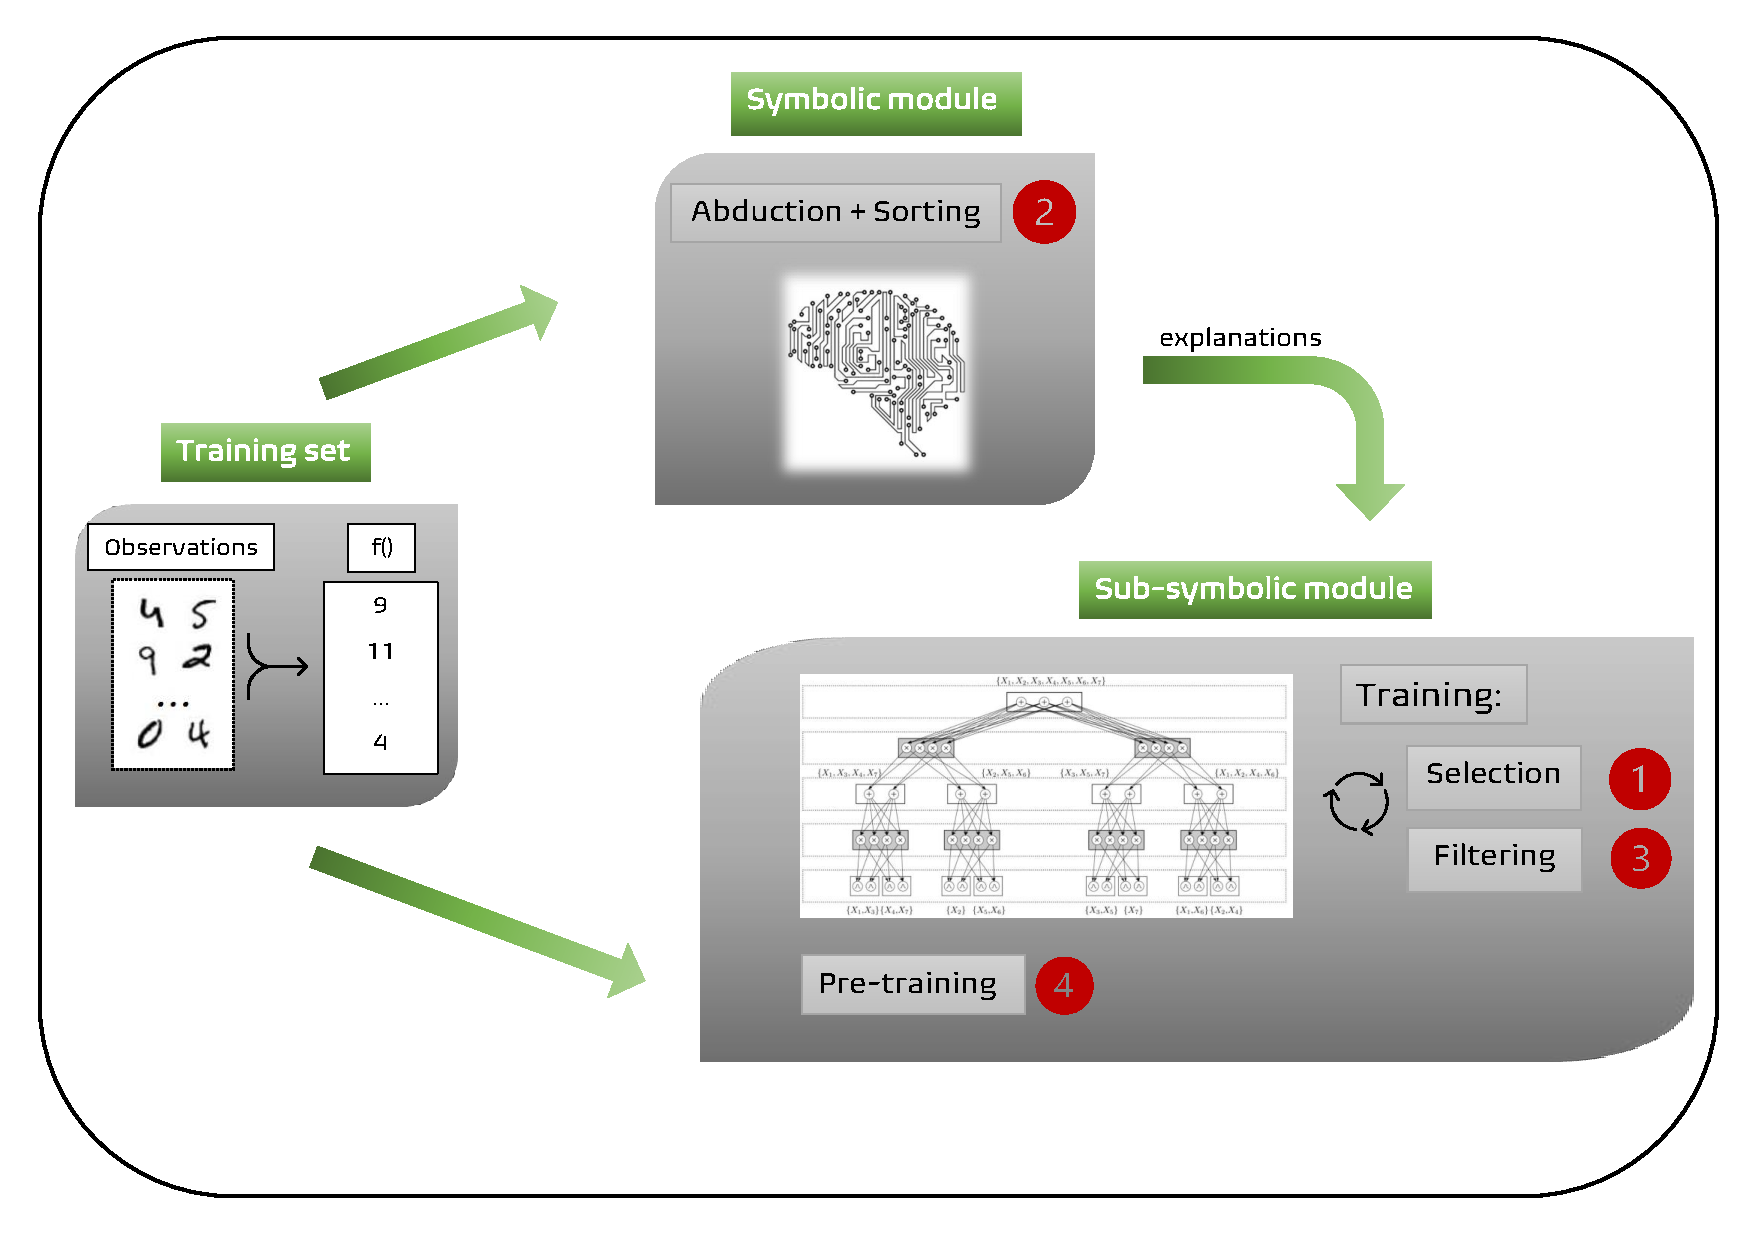
\includegraphics[scale=0.45]{Figures/architecture.pdf}
\end{figure}

\subsection{Abduction selection}
\label{abd-selection}
Since the function $\mathit{f}$ is not injective, the symbolic module suggests more than one possible abduction for each observation of the training set. The first key-point is to decide how to select the most suitable (ideally the correct) one in order to perform the training process. Let:

\begin{itemize}
	\item $\mathit{A}$ be the set of abductions returned by symbolic module for observations $\mathbf{x}_r,...,\mathbf{x}_{r+m} \in \mathit{X}$, where $\mathit{m}$ is $\mathit{f}$ arity;  
	\item $\mathit{a} = (\mathit{c_r^a},...,\mathit{c_{r+m}^a})$ be a generic element of $\mathit{A}$, such that labels $\mathit{c_r^a},...,\mathit{c_{r+m}^a}$ respectively correspond to observations $\mathbf{x}_r,...,\mathbf{x}_{r+m}$;
	\item $c$ be the classification function to be learned;
	\item $\theta$ be the set of RAT-SPN parameters;
\end{itemize}
The most probable abduction $a^*$ is the one that maximizes the joint probability that each considered observation is predicted by RAT-SPN as the suggested label. Since observations are supposed to be \textit{i.i.d.} (i.e., indipendent and identically distributed), the joint probability is computed as the product of single probabilities:
\begin{equation}\begin{split}
	a^* = \arg\max_{a \in \mathit{A}} p(\mathit{a}|\theta) &= \arg\max_{a \in \mathit{A}} p(c(\mathbf{x}_r) = c_r^a,...,c(\mathbf{x}_{r+m}) = c_{r+m}^a|\theta) \\
	&= \arg\max_{a \in \mathit{A}} \prod_{j=r}^{r+m} p(c(\mathbf{x}_j) = c_j^a|\theta)
\end{split}\end{equation}
Note that, since the considered probabilities depend on the RAT-SPN parameters, it is not said that the most probable abduction stays the same among the different training epochs (remember that RAT-SPN training works like neural networks one, see Section \ref{rat-spn}). Ideally, if the network is correctly learning, the selection will become more and more reliable (i.e., oriented to the correct labels) with incrasing epoch.

\subsection{Observations sorting}
\label{sorting}
Even if the function $\mathit{f}$ is not injective, it is not said that symbolic module assigns the same number of possible abduction to each observation and, moreover, some of them might have just one possible abduction. For example, let us consider the sum of a pair of digits from 0 to 9:

\begin{enumerate}[I.]
	\item if $sum(\mathit{c}_1,\mathit{c}_2) = 4$, then $\mathit{A} = \{(0,4), (1,3), (2,2), (3,1), (4,0)\}$ and $|A|=5$;
	\item if $sum(\mathit{c}_1,\mathit{c}_2) = 2$, then $\mathit{A} = \{(0,2), (1,1), (2,0)\}$ and $|A|=3$;
	\item if $sum(\mathit{c}_1,\mathit{c}_2) = 0$, then $\mathit{A} = \{(0,0)\}$ and $|A|=1$;
\end{enumerate}
The idea deriving from this observation is to ensure that, at each epoch, RAT-SPN performs the training on the observations sorted by their possible number of abductions. In this way, since the network is less good at classifying at the beginning of each epoch (i.e., for the first batches) rather than at the end, we try to reduce its possible choices at the beginning, trusting that it will perform better predictions going forward. With regard to the example above, observations would be sorted in the following way: III ($|A|=1$), II ($|A|=3$), I ($|A|=5$).

It is pointed out that such sorting is performed by the symbolic module, since it is striclty related to the abductive process; the sub-symbolic model just receives the possible abductions and the order in which it has to consider the observations during the training, ignoring the way in which this sorting has been performed.  

\subsection{Abduction threshold}
\label{abd-threshold}
The type of classification task we are dealing with (see Section \ref{classification}) is intrinsically characterized, by its nature, by a strong uncertainty factor. The labels selected by the sub-symbolic module among the ones suggested by the symbolic one might not always be correct, especially in the first training epochs when the model has not learned enough yet. Even if RAT-SPNs, as will be showed in Section \ref{results}, turn out to be very good at handling cases of mislabeling, we decided to provide a mechanism to filter the selected labels and consequently the corresponding observations from the training set, according to a specific certainty degree. Basically, the idea is to ensure that the model mainly learns from labels of which it is sufficienlty confident. Labels and observations are filtered on the basis of a value that essentially measures the probability difference between the first two most probable abductions. More precisely, let $a_1$ and $a_2$ be the first two probable abductions selected by the sub-symbolic module and respectively $p(a_1)$ and $p(a_2)$ be their probabilities computed by RAT-SPN; the value is calculated as follows:

\begin{equation}\
	v_{dif} = \frac{p(a_1)-p(a_2)}{p(a_1)} \times 100 
\end{equation}
If $v_{dif}$ is greater than the specified threshold (which is an hyper-parameter of the entire model), then the specific observations and the corresponding selected labels are used in the training process, as usual; otherwise, they are discarded. Naturally, it makes sense to use this threshold only when the possible number of abductions is strictly greater than 1. Note that, since $v_{dif}$ depends on the probability values returned by RAT-SPN, it is computed and compared again with the threshold at each epoch, because both $p(a_1)$, $p(a_2)$ and the same $a_1$, $a_2$ might be different. Therefore, it intuitively follows that the more the model learns the more observations will be considered, because it will become more and more good at disambiguating the observations. As we will see from the experiments, in a certain sense, increasing the threshold ensures a sort of "cool start", forcing the model to train from few examples especially in the first epochs, when it is more uncertain about the labels to choose. In some situations, depending on the specific classification task, this may result in starting to learn only from a subset of the labels (e.g., in the case of the sum of 2 digits, only from 0 and 9, since they correspond to the only certain labels), extending the training bit by bit to other classes.

\subsection{Pre-training}
\label{clustering}
In some situations it might happen that the number of observations for which the number of possible abductions is one (e.g., sum of two digits equal to zero) is not sufficient to allow the model to learn enough in order to be able to select the correct labels later, when the labeling is not as much certain. Nevertheless, if we know for sure the labels associated to some (even if few) observations, we can try in some way to look for other observations of the same class from the training set, on which to perform a \textit{pre-training} of the model and try to solve, at least partially, the initialization problem of RAT-SPN (which is totally randomic).

For this purpose, we decided to exploit the k-Means clustering \cite{macqueen1967}, or Lloyd’s algorithm \cite{1056489}, which is an iterative, data-partitioning algorithm that aims to partition $n$ observations into $k$ clusters in which each observation belongs to the cluster with the nearest mean (cluster centers or cluster centroid), serving as a prototype of the cluster. Naturally, k-Means doesn't provide the same performance of other more sophisticated algorithms, but, in this context, we are more interested in performing a fast clustering than a more accurate one, since our aim is just to initialize the model before the real training process.

Once the k-Means has been perfomed, given $m$ observations for which we know for sure that the label is $c$, we select the correspondent cluster, that is the one associated to observations. Since the correspondent cluster might not be unique, we perform a majority vote among the $m$ observations in order to choose the most frequent one; in case of equality, no cluster is selected for the pre-training. Hence, RAT-SPN is pre-trained for few epochs on the observations of the selected cluster, assigning them the label $c$, and then the real training starts as usual. 
\chapter{Experiments}
\label{ChapterExp}

The purpose of the current chapter is, in the first place, to describe in detail the specific tasks and datasets used for the experiments and, in the second place, to show and comment the obtained results.   

\section{Tasks and dataset}
\label{tasks-dataset}

In order to test the model depicted in Section \ref{arch-and-feat}, we considered the following task of the type described in Section \ref{classification}: learning to classify digits from 0 to 9, knowing the sum of $\mathit{n}$ tuples (having cardinality $\mathit{m}$) of them. With reference to the nomenclature used in Section \ref{classification}, let $\mathit{f} = sum(\mathit{c}_1,...,\mathit{c}_m)$ be the function that takes in input $\mathit{m}$ digits from 0 to 9 and compute their sums. Note that such function is not injective (e.g., if $m = 2: 0+3=3$ as well as $2+1=3$) and the order of the elements in the tuple is relevant in the interests of the classification task (e.g., if $m =2: (0,2) \neq (0,2)$ even if $\mathit{f}(0,2) = \mathit{f}(2,0) = 2$).

The starting dataset to perform this task is MNIST, that includes handwritten digits and it is commonly used for training and testing in the filed of machine learning. It contains 60'000 training images and 10'000 testing images; each image has 784 pixels ($28 \times 28$). For the purpose of the experiments, the training set has been split as follows: 54'000 examples for the training set and 6'000 for the validation set. Besides, we removed pixels with very low variance (in particular, where the pixel's variance is smaller than 0.001 times the average variance); the resulting images have 629 pixels. 

\begin{figure}[H]
\caption{Sample images from MNIST dataset.}
\label{fig:mnist}
\centering
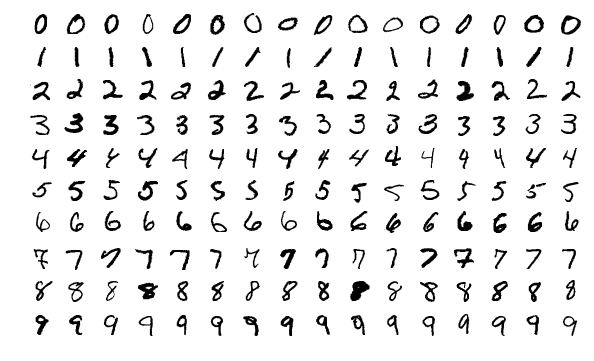
\includegraphics[scale=0.6]{Figures/mnist.png}
\end{figure}
Starting from the dataset just described, we applied the function $\mathit{f}$ to the labels $\mathit{c}_i \in \mathit{C}$ corresponding to observations $\mathbf{x}_i \in \mathit{X}$ in order to modify the dataset in the form $\{((\mathbf{x}_1,...,\mathbf{x}_m),\mathit{f}_1),...,((\mathbf{x}_{n-m+1},...,\mathbf{x}_n),\mathit{f}_{\frac{n}{m}})\}$. In particular, we considered 3 values of $\mathit{m}$ (i.e., number of addends in the sum): 2, 3 and 4. Increasing such a value makes the task harder for two reasons:

\begin{itemize}
  \item the number of possible abductions increases, with equal sum. For example: if $sum(\mathit{c}_1,\mathit{c}_2) = 2$, then $\mathit{A}$ = \{(0,2), (1,1), (2,0)\} and $|\mathit{A}| = 3$; if $sum(\mathit{c}_1,\mathit{c}_2,\mathit{c}_3) = 2$, then $\mathit{A}$ = \{(0,0,2), (0,2,0), (2,0,0), (1,1,0), (1,0,1), (0,1,1)\} and $|\mathit{A}| = 6$;
  \item the number of observed cases in the modified dataset in which there is only one possible abduction decreases. In order to explain this observation, let us first consider the case of $m = 2$. The cases in which we have just one possible abduction are when the sum is 0 or 18; in fact, in such cases, we know that the possible addends are respectively only (0,0) and (9,9). Considering $m = 3$, we can make the same argument for sums 0 and 27. The difference lies in the way in which the modified dataset is computed: since we apply the function $\mathit{f} = sum(\mathit{c}_1,...,\mathit{c}_m)$ to the labels $\mathit{c}_i \in \mathit{C}$, the cases in which we have $m = 3$ zero (or equivalently nine) in succession decreases. Similarly, this number goes on to decrease when we consider $m = 4$.
\end{itemize}
Basically, we want to evaluate the model making the task more and more difficult, that is decreasing the number of observed certainties (i.e., cases in which there is only one possible abduction) and increasing the number of possible abductions. 
 
These considerations are highlighted in Table \ref{tab:info-tasks}, which shows the number of examples and the corresponding number of possible abductions by varying the value of $m$. We can observe that the certainties decrease from 1048 when $m = 2$ to 102 when $m = 3$ to only 12 when $m = 4$. Besides, we underline the significative increse of possible abductions for examples.

\begin{table}[H]
  \centering
  \caption{Number of examples and corresponding number of possible abductions respectively for $m = 2$, $m = 3$ and $m = 4$ for dataset MNIST. Rows in bold highlight the certainties for each task.}
  \label{tab:info-tasks}
  \scriptsize
  \begin{tabular}[t]{ll}
    \toprule
    \#(ex)	& \#(abd)\\
    \midrule
    \textbf{1048}	& \textbf{1}\\
    2480			& 2\\
	3228			& 3\\
	4580			& 4\\
	5278			& 5\\
	6398			& 6\\
	7332			& 7\\
	8640			& 8\\
	9744			& 9\\
	5272			& 10\\
    \bottomrule
  \end{tabular}
  \qquad
  \scriptsize
  \begin{tabular}[t]{ll}
    \toprule
    \#(ex)	& \#(abd)\\
    \midrule
    \textbf{102}	& \textbf{1}\\
    459				& 3\\
	684				& 6\\
	1305			& 10\\
	1788			& 15\\
	2625			& 21\\
	2961			& 28\\
	3927			& 36\\
	4803			& 45\\
	5952			& 55\\
	6585			& 63\\
	7269			& 69\\
	7707			& 73\\
	7833			& 75\\
    \bottomrule
  \end{tabular}
    \qquad
  \scriptsize
  \begin{tabular}[t]{ll}
    \toprule
    \#(ex)	& \#(abd)\\
    \midrule
    \textbf{12}		& \textbf{1}\\
    40				& 4\\
	164				& 10\\
	296				& 20\\
	412				& 35\\
	708				& 56\\
	1104			& 84\\
	1468			& 120\\
	1836			& 165\\
	2452			& 220\\
	3164			& 282\\
	3776			& 348\\
	4556			& 415\\
	5288			& 480\\
	5824			& 540\\
	6484			& 592\\
	6336			& 633\\
	6636			& 660\\
	3444			& 670\\
    \bottomrule
  \end{tabular}
\end{table}

\section{Results}
\label{results}
In the following, we show and analyse the experiments results on the tree tasks described in Section \ref{tasks-dataset}. According to the specific task and related difficulties, we performed a grid search by varying the model hyper-parameters, which are in summary:

\begin{itemize}
	\item split-depth, number of input distributions, number of root nodes, number of sum nodes per inner regions, dropout at input, dropout at sums (from RAT-SPN, see Section \ref{rat-spn});
	\item abductions threshold and pre-training (see Sections \ref{abd-threshold} and \ref{clustering}).
\end{itemize}
On the contrary, we fixed the batch size and the number of epochs to $100$ and the use of \textit{adam} (adaptive moment estimation) \cite{kingma2017adam} as optimization algorithm for RAT-SPN.

\subsection{Sum of pairs}
\label{results-pairs}
Table \ref{tab:results-pairs} shows the esperiments results in the case of $m=2$ (i.e., sum of pairs). Because of the training computational cost of RAT-SPNs with split depth striclty greater than 1, we tested only the configurations with split depth equal to 1, exploring almost all the ones proposed by Peharz et al. \cite{DBLP:journals/corr/abs-1806-01910} in the original experiments on mnist dataset (only configurations with dropout equal to 0.25 have been discarded, given th reduced dimension of the considered SPNs). As regards the introduced hyper-parameters (i.e., abduction threshold and pre-training), since the task under consideration presents a sufficiently high number of "certainties" (i.e., observations with just one possible abduction) and a not so significant number of possible abductions (see Table \ref{tab:info-tasks}), we decided not to exploit these additional implemented features in this case (i.e., threshold = 0 and pre-training = false).

\begin{table}[H]
  \centering
  \caption{Performance for $\mathit{f} = sum(\mathit{c}_1,\mathit{c}_2)$. Batch size = $100$, number of epochs = $100$, optimization algorithm: \textit{adam}, abductions threshold = 0, pre-training = false. All accuracy values are in percentage and approximated to the second digit after the decimal place. The best configuration is highlighted in bold.}
  \label{tab:results-pairs}
  \tiny
  \begin{tabular}{ccccccrr}
    \toprule
    depth		& distributions 	& splits 		& sums 				& dropout input 		& dropout sums 			& valid acc 			& test acc\\
    \midrule
    1      		& 10     			& 9      		& 10     			& 1      				& 1      				& 94.87    				& 94.74\\ 
    1      		& 10     			& 9      		& 10     			& 1      				& 0.75    				& 94.77    				& 94.8\\ 
    1      		& 10     			& 9      		& 10     			& 1      				& 0.50    				& 95.27    				& 94.84\\	
	1      		& 10     			& 9      		& 10     			& 0.75    				& 1      				& 96.07    				& 95.77\\
	1      		& 10     			& 9      		& 10     			& 0.75    				& 0.75    			    & 96.18    				& 95.76\\         
    1      		& 10     			& 9      		& 10     			& 0.75    				& 0.50    				& 96.53    				& 95.91\\ 
    1      		& 10     			& 9      		& 10     			& 0.50    				& 1      				& 96.17				    & 95.89\\
	1      		& 10     			& 9      		& 10     			& 0.50    				& 0.75    				& 96.38    				& 95.90\\   
    1      		& 10				& 9			    & 10				& 0.50					& 0.50					& 96.07    				& 95.82\\
 
	1      		& 15     			& 14     		& 10     			& 1      				& 1      				& 94.90				    & 95.43\\ 
	1      		& 15     			& 14     		& 10     			& 1      				& 0.75    				& 95.57    				& 95.57\\
	1      		& 15     			& 14     		& 10     			& 1      				& 0.50    				& 95.12    				& 95.30\\ 
	1      		& 15     			& 14     		& 10     			& 0.75    				& 1      				& 96.57				    & 96.23\\  
	1      		& 15     			& 14     		& 10     			& 0.75    				& 0.75    				& 96.48    				& 96.36\\
	1      		& 15     			& 14     		& 10     			& 0.75   	 			& 0.50    				& 96.72    				& 96.27\\ 
	1      		& 15     			& 14     		& 10     			& 0.50    				& 1      			    & 96.53    				& 96.08\\
	1      		& 15     			& 14     		& 10     			& 0.50    				& 0.75    				& 96.63    				& 96.17\\  
	1      		& 15     			& 14     		& 10     			& 0.50    				& 0.50    				& 96.33    				& 95.99\\ 

	1      		& 20     			& 19     		& 10     			& 1      				& 1      				& 95.60    				& 95.59\\ 
	1      		& 20     			& 19     		& 10     			& 1      				& 0.75					& 95.37				    & 95.45\\ 
	1      		& 20     			& 19     		& 10     			& 1      				& 0.50					& 95.63    				& 95.22\\
	1      		& 20     			& 19     		& 10     			& 0.75    				& 1     				& 96.88    				& 96.58\\  
	1		    & 20     			& 19     		& 10     			& 0.75    				& 0.75				    & 96.60    				& 96.47\\ 
	1      		& 20     			& 19     		& 10     			& 0.75    				& 0.50    				& 96.57					& 96.67\\
	1      		& 20     			& 19     		& 10     			& 0.50    				& 1						& 96.95   				& 96.48\\ 
	1      		& 20     			& 19     		& 10     			& 0.50    				& 0.75    				& 96.52    				& 96.28\\ 
	1      		& 20     			& 19     		& 10     			& 0.50    				& 0.50    				& 96.75    				& 96.19\\ 

	1      		& 25     			& 29     		& 10     			& 1      				& 1      				& 95.90    				& 95.80\\
	1	      	& 25     			& 29     		& 10     			& 1      				& 0.75    				& 95.83    				& 95.73\\
	1      		& 25     			& 29     		& 10     			& 1      				& 0.50    				& 95.62					& 95.90\\
	1      		& 25     			& 29     		& 10     			& 0.75    				& 1      				& 96.93    				& 96.51\\
 	1      		& 25     			& 29     		& 10     			& 0.75    				& 0.75    				& 96.72    				& 96.63\\ 
	1      		& 25     			& 29     		& 10     			& 0.75    				& 0.50    				& 96.87					& 96.76\\
	1      		& 25     			& 29     		& 10     			& 0.50    				& 1      				& 96.82    				& 96.73\\ 
	1      		& 25     			& 29     		& 10     			& 0.50    				& 0.75    				& 96.95				    & 96.60\\
	1      		& 25     			& 29     		& 10     			& 0.50   				& 0.50    				& 96.67				    & 96.50\\

	1      		& 33     			& 40     		& 10     			& 1      				& 1      				& 95.97    				& 95.67\\
	1      		& 33     			& 40     		& 10     			& 1      				& 0.75    				& 95.78    				& 95.93\\
	1      		& 33     			& 40     		& 10     			& 1      				& 0.50    				& 95.77    				& 95.71\\
	1      		& 33    			& 40     		& 10     			& 0.75    				& 1      				& 96.77    				& 96.51\\
	1      		& 33     			& 40    		& 10     			& 0.75    				& 0.75    				& 96.77    				& 96.66\\ 	
	1      		& 33     			& 40     		& 10     			& 0.75				    & 0.50				    & 96.90				    & 96.48\\ 
	1      		& 33     			& 40     		& 10     			& 0.50    				& 1      				& 97.03    				& 96.89\\ 
	1      		& 33     			& 40     		& 10     			& 0.50    				& 0.75					& 96.95					& 96.87\\ 			
	\textbf{1} 	& \textbf{33}     	& \textbf{40}   & \textbf{10}		& \textbf{0.50}    		& \textbf{0.50}    		& \textbf{97.10}    	& \textbf{96.88}\\
    \bottomrule
  \end{tabular}
\end{table}

\newpage
First of all, we observe that accuracy values are very similar among all the considered configurations, in contrast with the model showed in Section \ref{challenge}. This means that the labeling accuracy (hence the training success) does not depend on the chance, but on a deterministic learning, that always carries out the model to understand (more or less according to the specific configuration and only in a very small part to the chance) the proper "direction" to take. In conclusion, we can infer that, for this specific task, the only observations sorting mechanism (described in Section \ref{sorting}) turns out to be sufficient in order to achieve great performance.

\subsection{Sum of triples}
Table \ref{tab:results-triples-clno} and \ref{tab:results-triples-clyes} show the esperiments results in the case of $m=3$ (i.e., sum of triples). Since in the previous experiment (Section \ref{results-pairs}) no significant difference was observed increasing the number of input distributions and since we are more interested in understanding the model behaviour than the real performance in terms of accuracy, we explored the ones having less computational cost. In this case, however, given the increased difficulty (see Table \ref{tab:info-tasks}) we introduced both the abduction threshold and the pre-training. 

\begin{table}[H]
  \centering
  \caption{Performance for $\mathit{f} = sum(\mathit{c}_1,\mathit{c}_2,\mathit{c}_3)$. Batch size = $100$, number of epochs = $100$, optimization algorithm: \textit{adam}, \textbf{pre-training = false}. All accuracy values are in percentage and approximated to the second digit after the decimal place. The best configuration is highlighted in bold.}
  \label{tab:results-triples-clno}
  \scriptsize
  \begin{tabular}{cccccccrr}
    \toprule
    depth		& distributions 	& splits 		& sums 				& dropout input 		& dropout sums 			& threshold				& valid acc 			& test acc\\
    \midrule
	1      		& 10     			& 9      		& 10     			& 1      				& 1      				& 0      				& 94.10    				& 94.19\\ 
	1      		& 10     			& 9				& 10     			& 1      				& 1      				& 0.01    				& 98.05    			    & 94.22\\ 
	1      		& 10     			& 9      		& 10     			& 1      				& 1      				& 0.05    				& 94.47    				& 94.30\\
	1      		& 10     			& 9      		& 10     			& 1      				& 1      				& 0.10    				& 94.35    				& 94.35\\
    1      		& 10     			& 9      		& 10     			& 0.75    				& 0.75    				& 0      				& 96.78    				& 96.46\\
	1      		& 10     			& 9      		& 10     			& 0.75    				& 0.75    				& 0.05    				& 96.27    				& 95.89\\
	1      		& 10     			& 9      		& 10     			& 0.75    				& 0.75    				& 0.01    				& 96.63    				& 96.21\\ 
	1      		& 10     			& 9      		& 10     			& 0.75    				& 0.75    				& 0.10    				& 95.82    				& 95.45\\ 

	1      		& 15     			& 14     		& 10     			& 1      				& 1      				& 0      				& 94.22    				& 94.52\\
	1      		& 15     			& 14     		& 10     			& 1      				& 1      				& 0.01    				& 95.23    				& 94.63\\ 		
	1      		& 15     			& 14     		& 10     			& 1      				& 1      				& 0.05    				& 94.67    				& 94.66\\
	1      		& 15     			& 14     		& 10     			& 1      				& 1      				& 0.10    				& 98.14					& 94.71\\
	1      		& 15     			& 14     		& 10     			& 0.75    				& 0.75    				& 0      				& 96.85					& 96.14\\ 
	1      		& 15     			& 14     		& 10     			& 0.75					& 0.75					& 0.01					& 96.00    				& 95.57\\ 
	1      		& 15     			& 14     		& 10     			& 0.75    				& 0.75    				& 0.05    				& 96.63    				& 96.34\\ 
	1      		& 15     			& 14     		& 10     			& 0.75    				& 0.75    				& 0.10    				& 95.52    				& 95.49\\ 

	\textbf{1}  & \textbf{20}     	& \textbf{19}	& \textbf{10}		& \textbf{1}			& \textbf{1}      		& \textbf{0}      		& \textbf{98.52} 		& \textbf{94.78}\\ 
	1      		& 20     			& 19     		& 10     			& 1      				& 1      				& 0.01    				& 94.73    				& 94.59\\ 
	1      		& 20     			& 19     		& 10     			& 1      				& 1      				& 0.05    				& 94.62    				& 94.68\\
	1      		& 20     			& 19     		& 10     			& 1      				& 1      				& 0.10    				& 95.13    				& 94.66\\
	1      		& 20     			& 19     		& 10     			& 0.75      			& 0.75      			& 0	    				& 96.27    				& 96.10\\
	1      		& 20     			& 19     		& 10     			& 0.75      			& 0.75      			& 0.01    				& 96.87    				& 96.29\\
	1      		& 20     			& 19     		& 10     			& 0.75      			& 0.75      			& 0.05    				& 96.63    				& 96.35\\
	1      		& 20     			& 19     		& 10     			& 0.75      			& 0.75      			& 0.10    				& 96.83    				& 96.58\\
    \bottomrule
  \end{tabular}
\end{table}

\begin{table}[H]
  \centering
  \caption{Performance for $\mathit{f} = sum(\mathit{c}_1,\mathit{c}_2,\mathit{c}_3)$. Batch size = $100$, number of epochs = $100$, optimization algorithm: \textit{adam}, \textbf{pre-training = true}. All accuracy values are in percentage and approximated to the second digit after the decimal place. The best configuration is highlighted in bold.}
  \label{tab:results-triples-clyes}
  \scriptsize
  \begin{tabular}{cccccccrr}
    \toprule
    depth		& distributions 	& splits 		& sums 				& dropout input 		& dropout sums 			& threshold				& valid acc 			& test acc\\
    \midrule
	1      		& 10     			& 9      		& 10     			& 1      				& 1      				& 0      				& 94.05    				& 94.23\\ 
	1      		& 10     			& 9				& 10     			& 1      				& 1      				& 0.01    				& 94.65    			    & 94.24\\ 
	1      		& 10     			& 9      		& 10     			& 1      				& 1      				& 0.05    				& 94.17    				& 94.37\\
	1      		& 10     			& 9      		& 10     			& 1      				& 1      				& 0.10    				& 94.23    				& 94.02\\
    1      		& 10     			& 9      		& 10     			& 0.75    				& 0.75    				& 0      				& 96.50    				& 95.87\\
	1      		& 10     			& 9      		& 10     			& 0.75    				& 0.75    				& 0.05    				& 96.32    				& 95.96\\
	1      		& 10     			& 9      		& 10     			& 0.75    				& 0.75    				& 0.01    				& 96.38    				& 96.08\\ 
	1      		& 10     			& 9      		& 10     			& 0.75    				& 0.75    				& 0.10    				& 96.08    				& 95.86\\ 

	1      		& 15     			& 14     		& 10     			& 1      				& 1      				& 0      				& 94.80   				& 94.79\\
	1      		& 15     			& 14     		& 10     			& 1      				& 1      				& 0.01    				& 95.00    				& 94.96\\ 		
	1      		& 15     			& 14     		& 10     			& 1      				& 1      				& 0.05    				& 95.02    				& 94.92\\
	1      		& 15     			& 14     		& 10     			& 1      				& 1      				& 0.10    				& 94.43					& 94.08\\
	1      		& 15     			& 14     		& 10     			& 0.75    				& 0.75    				& 0      				& 96.80					& 96.25\\ 
	1      		& 15     			& 14     		& 10     			& 0.75					& 0.75					& 0.01					& 96.37    				& 95.41\\ 
	1      		& 15     			& 14     		& 10     			& 0.75    				& 0.75    				& 0.05    				& 96.57    				& 96.13\\ 
	1      		& 15     			& 14     		& 10     			& 0.75    				& 0.75    				& 0.10    				& 96.57    				& 96.40\\ 

	1  			& 20     			& 19			& 10				& 1						& 1      				& 0      				& 95.13 				& 94.59\\ 
	1      		& 20     			& 19     		& 10     			& 1      				& 1      				& 0.01    				& 94.88    				& 95.26\\ 
	1      		& 20     			& 19     		& 10     			& 1      				& 1      				& 0.05    				& 95.02    				& 95.14\\
	1      		& 20     			& 19     		& 10     			& 1      				& 1      				& 0.10    				& 95.13    				& 94.87\\
	\textbf{1}  & \textbf{20}     	& \textbf{19}   & \textbf{10}     	& \textbf{0.75}      	& \textbf{0.75}      	& \textbf{0}	    	& \textbf{96.88}    	& \textbf{96.15}\\
	1      		& 20     			& 19     		& 10     			& 0.75      			& 0.75      			& 0.01    				& 96.82    				& 96.38\\
	1      		& 20     			& 19     		& 10     			& 0.75      			& 0.75      			& 0.05    				& 96.70    				& 96.47\\
	1      		& 20     			& 19     		& 10     			& 0.75      			& 0.75      			& 0.10    				& 96.80    				& 96.45\\
    \bottomrule
  \end{tabular}
\end{table}
As with the case of $m=2$, we can notice the same constant behaviour (in terms of accuracy) among the tested configurations. Such consideration confirms that, also in the case of a task that is more difficult than the previous one, the learning process is deterministic. As regards the abduction threshold, its use doesn't seem to bring advantages to the model, from a purely perfomance point of view; the best observed configurations (highlighted in bold) actually work without threshold (i.e., equal to 0). Analogous observation can be done for the pre-training: even if the best configuration of the pre-trained model performs better on the test set with respect to the best of the not pre-trained one, the comparison between correspondent configurations points out a substancial similarity. Nevertheless, it is interesting to see if some differences come out in the general model behaviour by varying the threshold value and enabling the pre-training. To this end, Figures \ref{fig:thresholds-triples} show \textit{(i)} the number of considered examples, \textit{(ii)} the examples labeling accuracy (to perform the successive training) and \textit{(iii)} the model accuracy on validation set per epoch, by varying the abduction threshold and enabling the pre-training. We can make the following observations:

\begin{itemize}
	\item the greater the threshold, the more the number of considered examples increases slowly; of course, when the threshold is equal to 0, all examples are taken into account from the first epoch to the last one. Besides, when the pre-training is enabled, much more examples are considered from the beginning and the number of considered examples increases faster, since the initialization of the model is no longer randomic;
	\item in the case of threshold uqual to 0.05 and 0.1 without pre-training, the examples labeling accuracy starts from the top value (since it considers all and only the examples with just one possible abduction), but then it drops to very small values, because the low number of considered examples was not sufficient to learn enough. Nevertheless, in both cases, the model is able to improve again its examples labeling accuracy and to easily overcome the model without threshold (i.e., equal to 0) after some epochs. When pre-training is enabled, the model directly starts from low values of labeling accuracy, since it considers more examples from the beginning, and it again learns faster than the model wituout threshold. The motivation behind such improvement definitely lies in the fact the such threshold values allow the model to label (and consequenlty consider) examples with a certain degree of certainty. On the contrary, when the threshold is set to 0.01, no advantage is observed, actually the no threshold model performs better;
	\item the model accuracy behaviour on validation set is very similar to the examples labeling accuracy one (except for the drop in the case of thresholds 0.05 and 0.1 and disabled pre-training). The motivation of such observation lies in the way in which the most probable abduction is selected (see \ref{abd-selection}): since this choice depends on the sub-symbolic model, the more it is learning, the more its accuracy increases both on the validation set and in selecting the abduction for the training examples.
\end{itemize}
In the light of the above considerations, we can conclude that, although all configurations achieve good performance in terms of accuracy, the use both of a sufficiently high threshold and of the pre-training allows the model to converge faster, even if starting from lower accuracy values.

\begin{figure}[H]
\captionsetup{font={small, stretch=1.3}}
\caption{Behaviour comparison between the not pre-trained model and the pre-trained one for $\mathit{f} = sum(\mathit{c}_1,\mathit{c}_2,\mathit{c}_3)$, taking into account: number of considered examples, examples labeling accuracy and model accuracy on validation set per epoch by varying the abduction threshold. The average values have been computed among different configurations but with the same threshold.}
\label{fig:thresholds-triples}
{\setlength{\tabcolsep}{1pt}
\renewcommand*{\arraystretch}{0.6}
\begin{longtable}{cc}
\textbf{Pre-training = false} & \textbf{Pre-training = true} \\
\subfloat{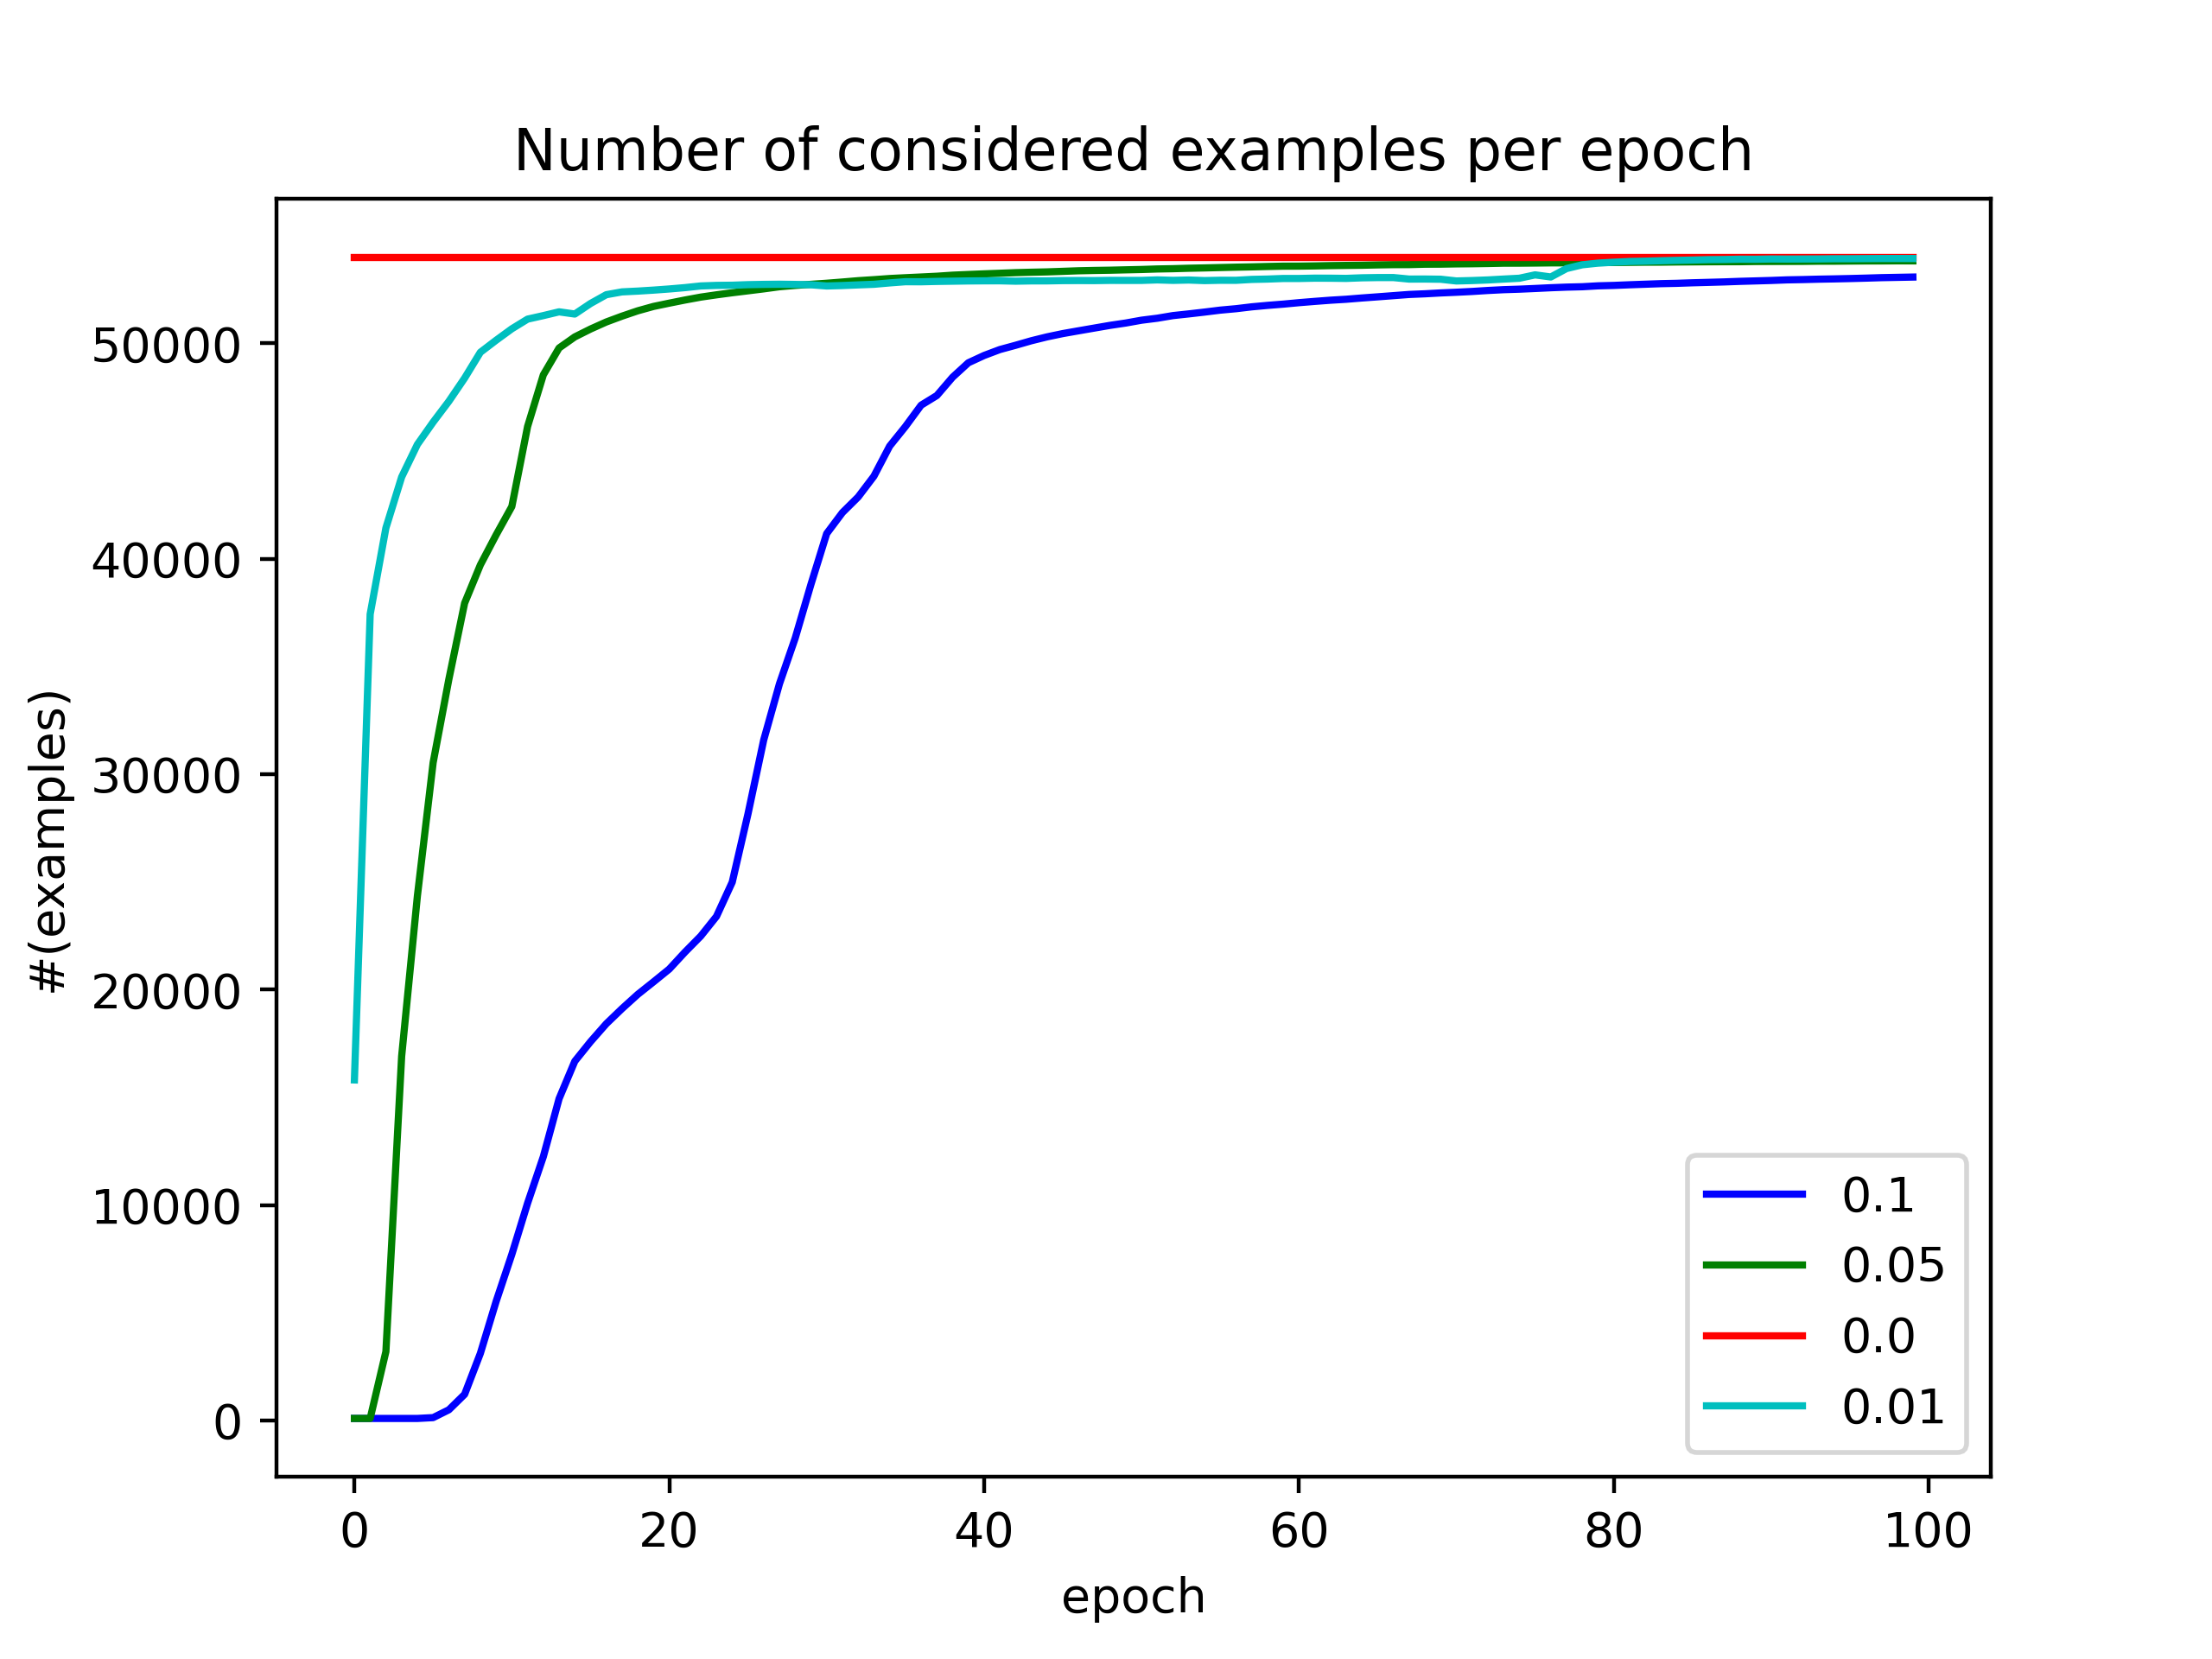
\includegraphics[scale=0.45]{Figures/num_addends_3/examples_clno.png}} & 
\subfloat{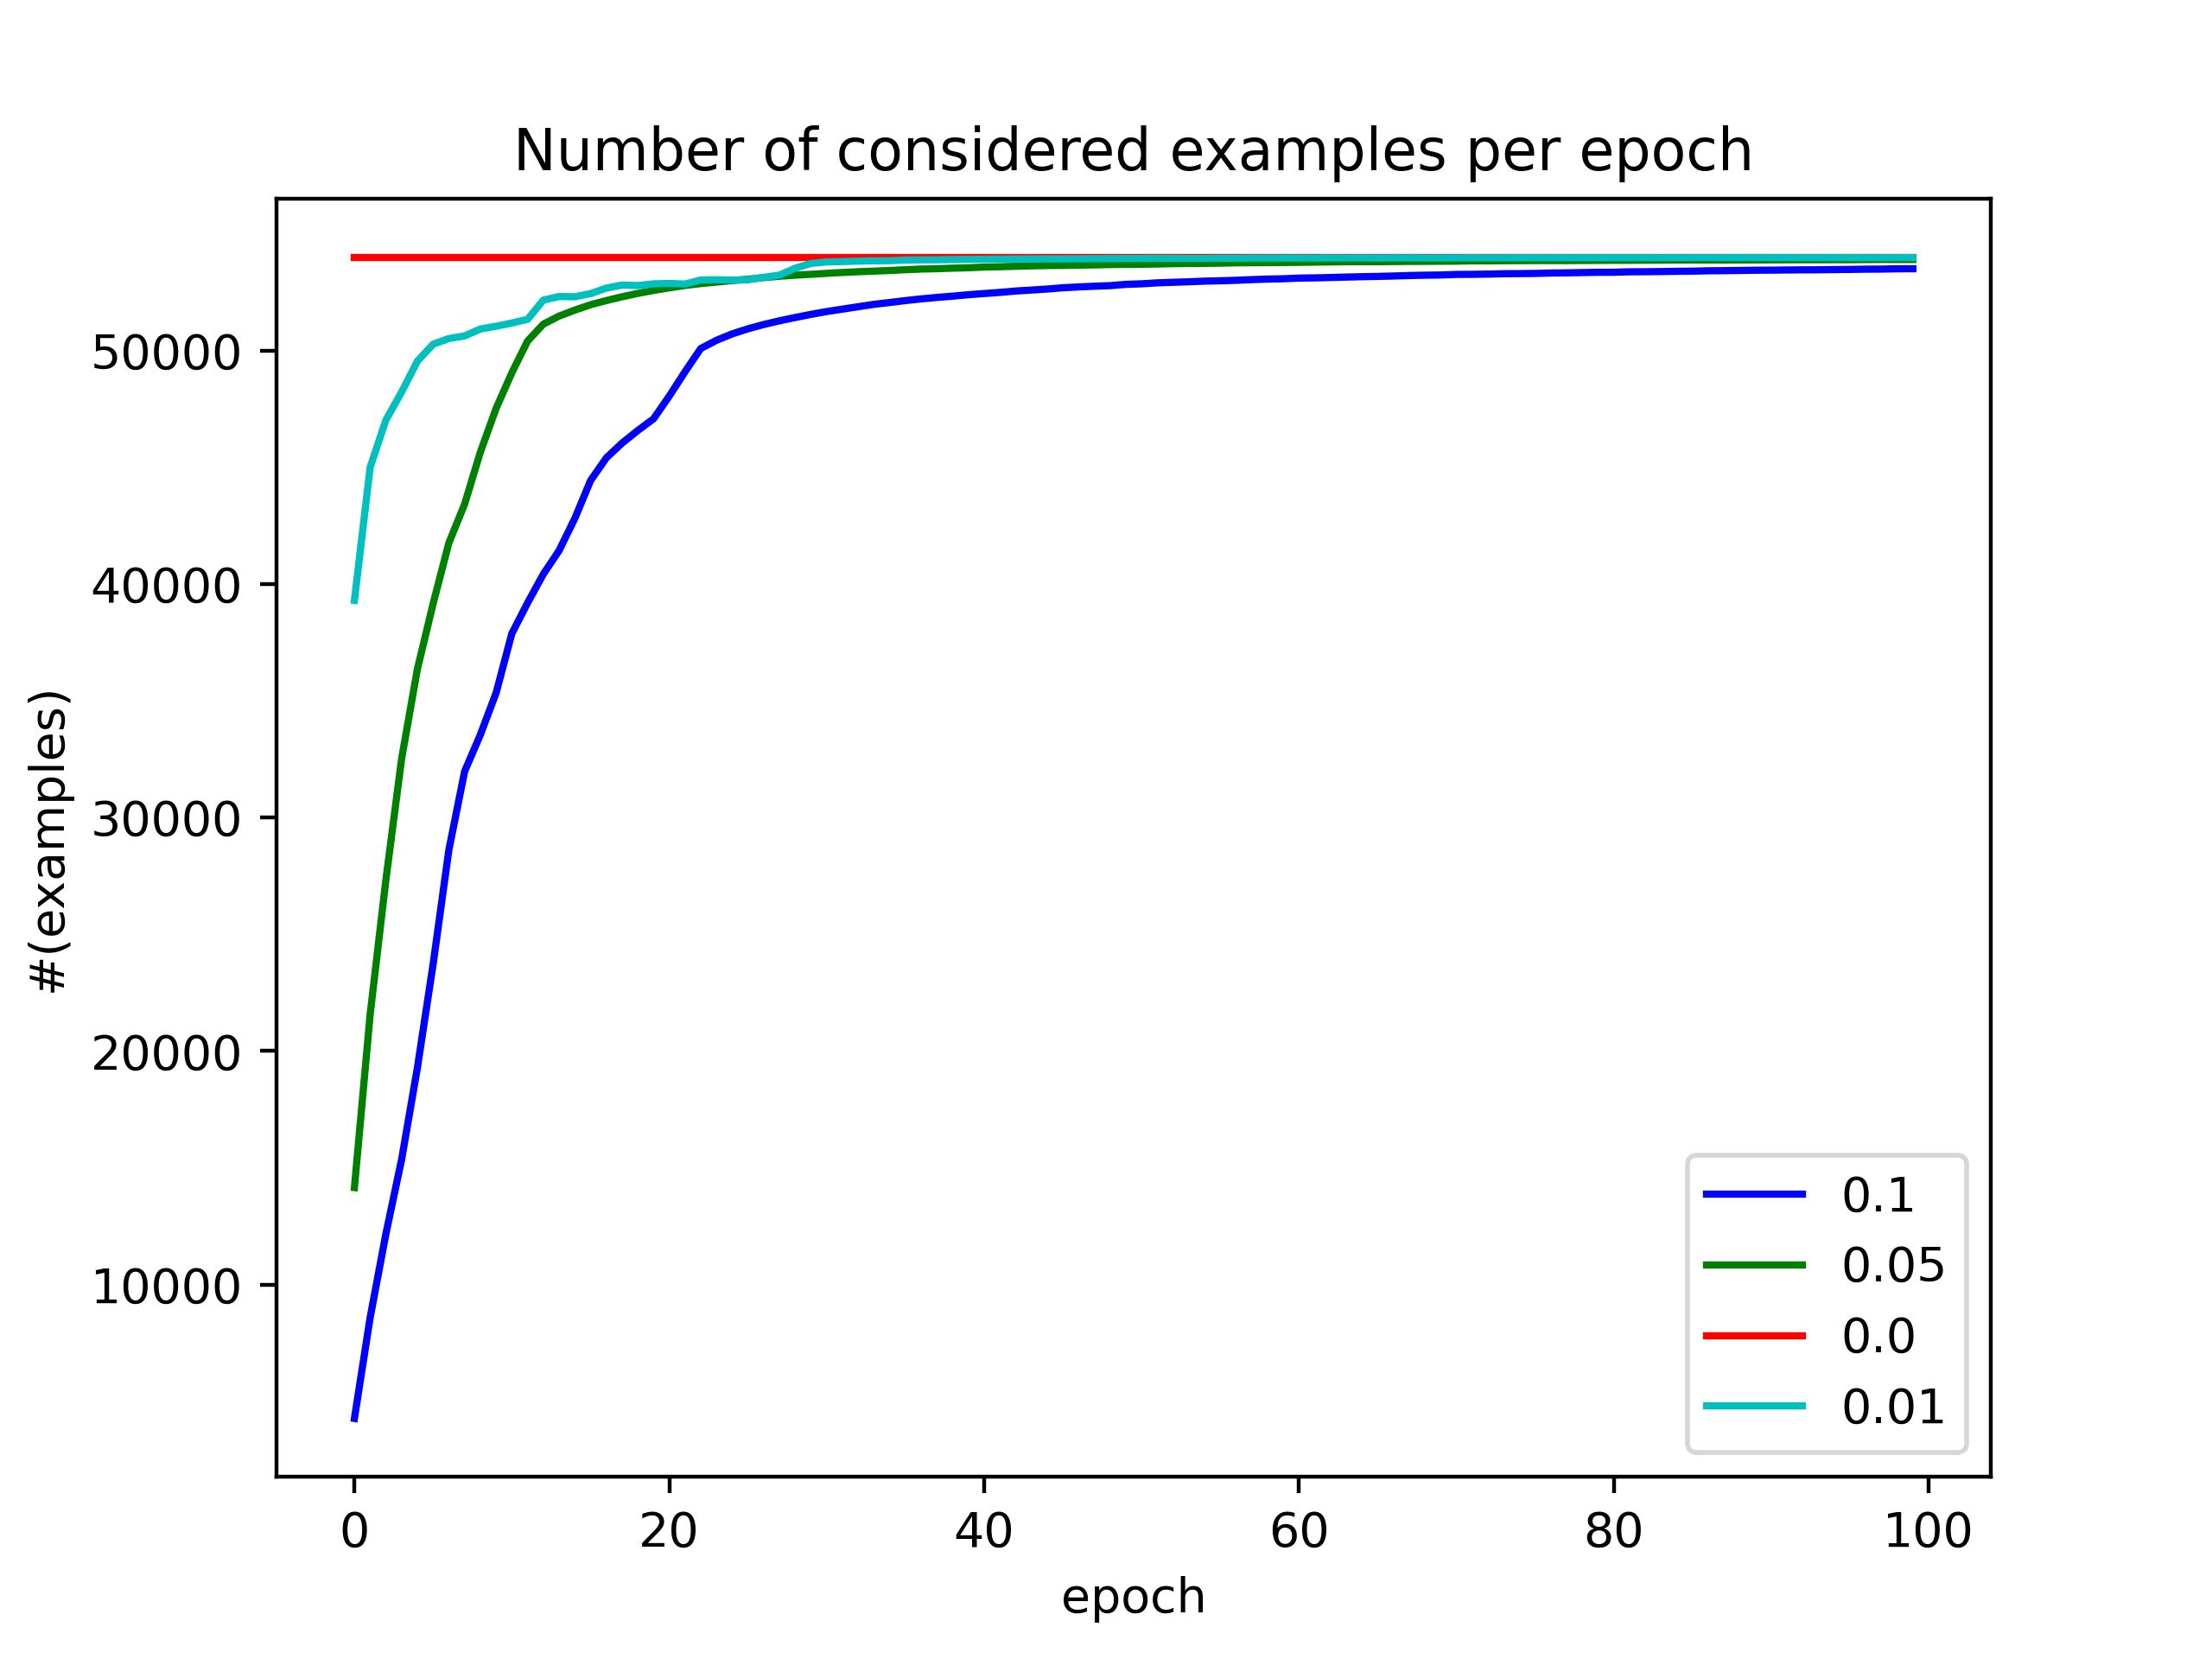
\includegraphics[scale=0.45]{Figures/num_addends_3/examples_clyes.png}} \\

\subfloat{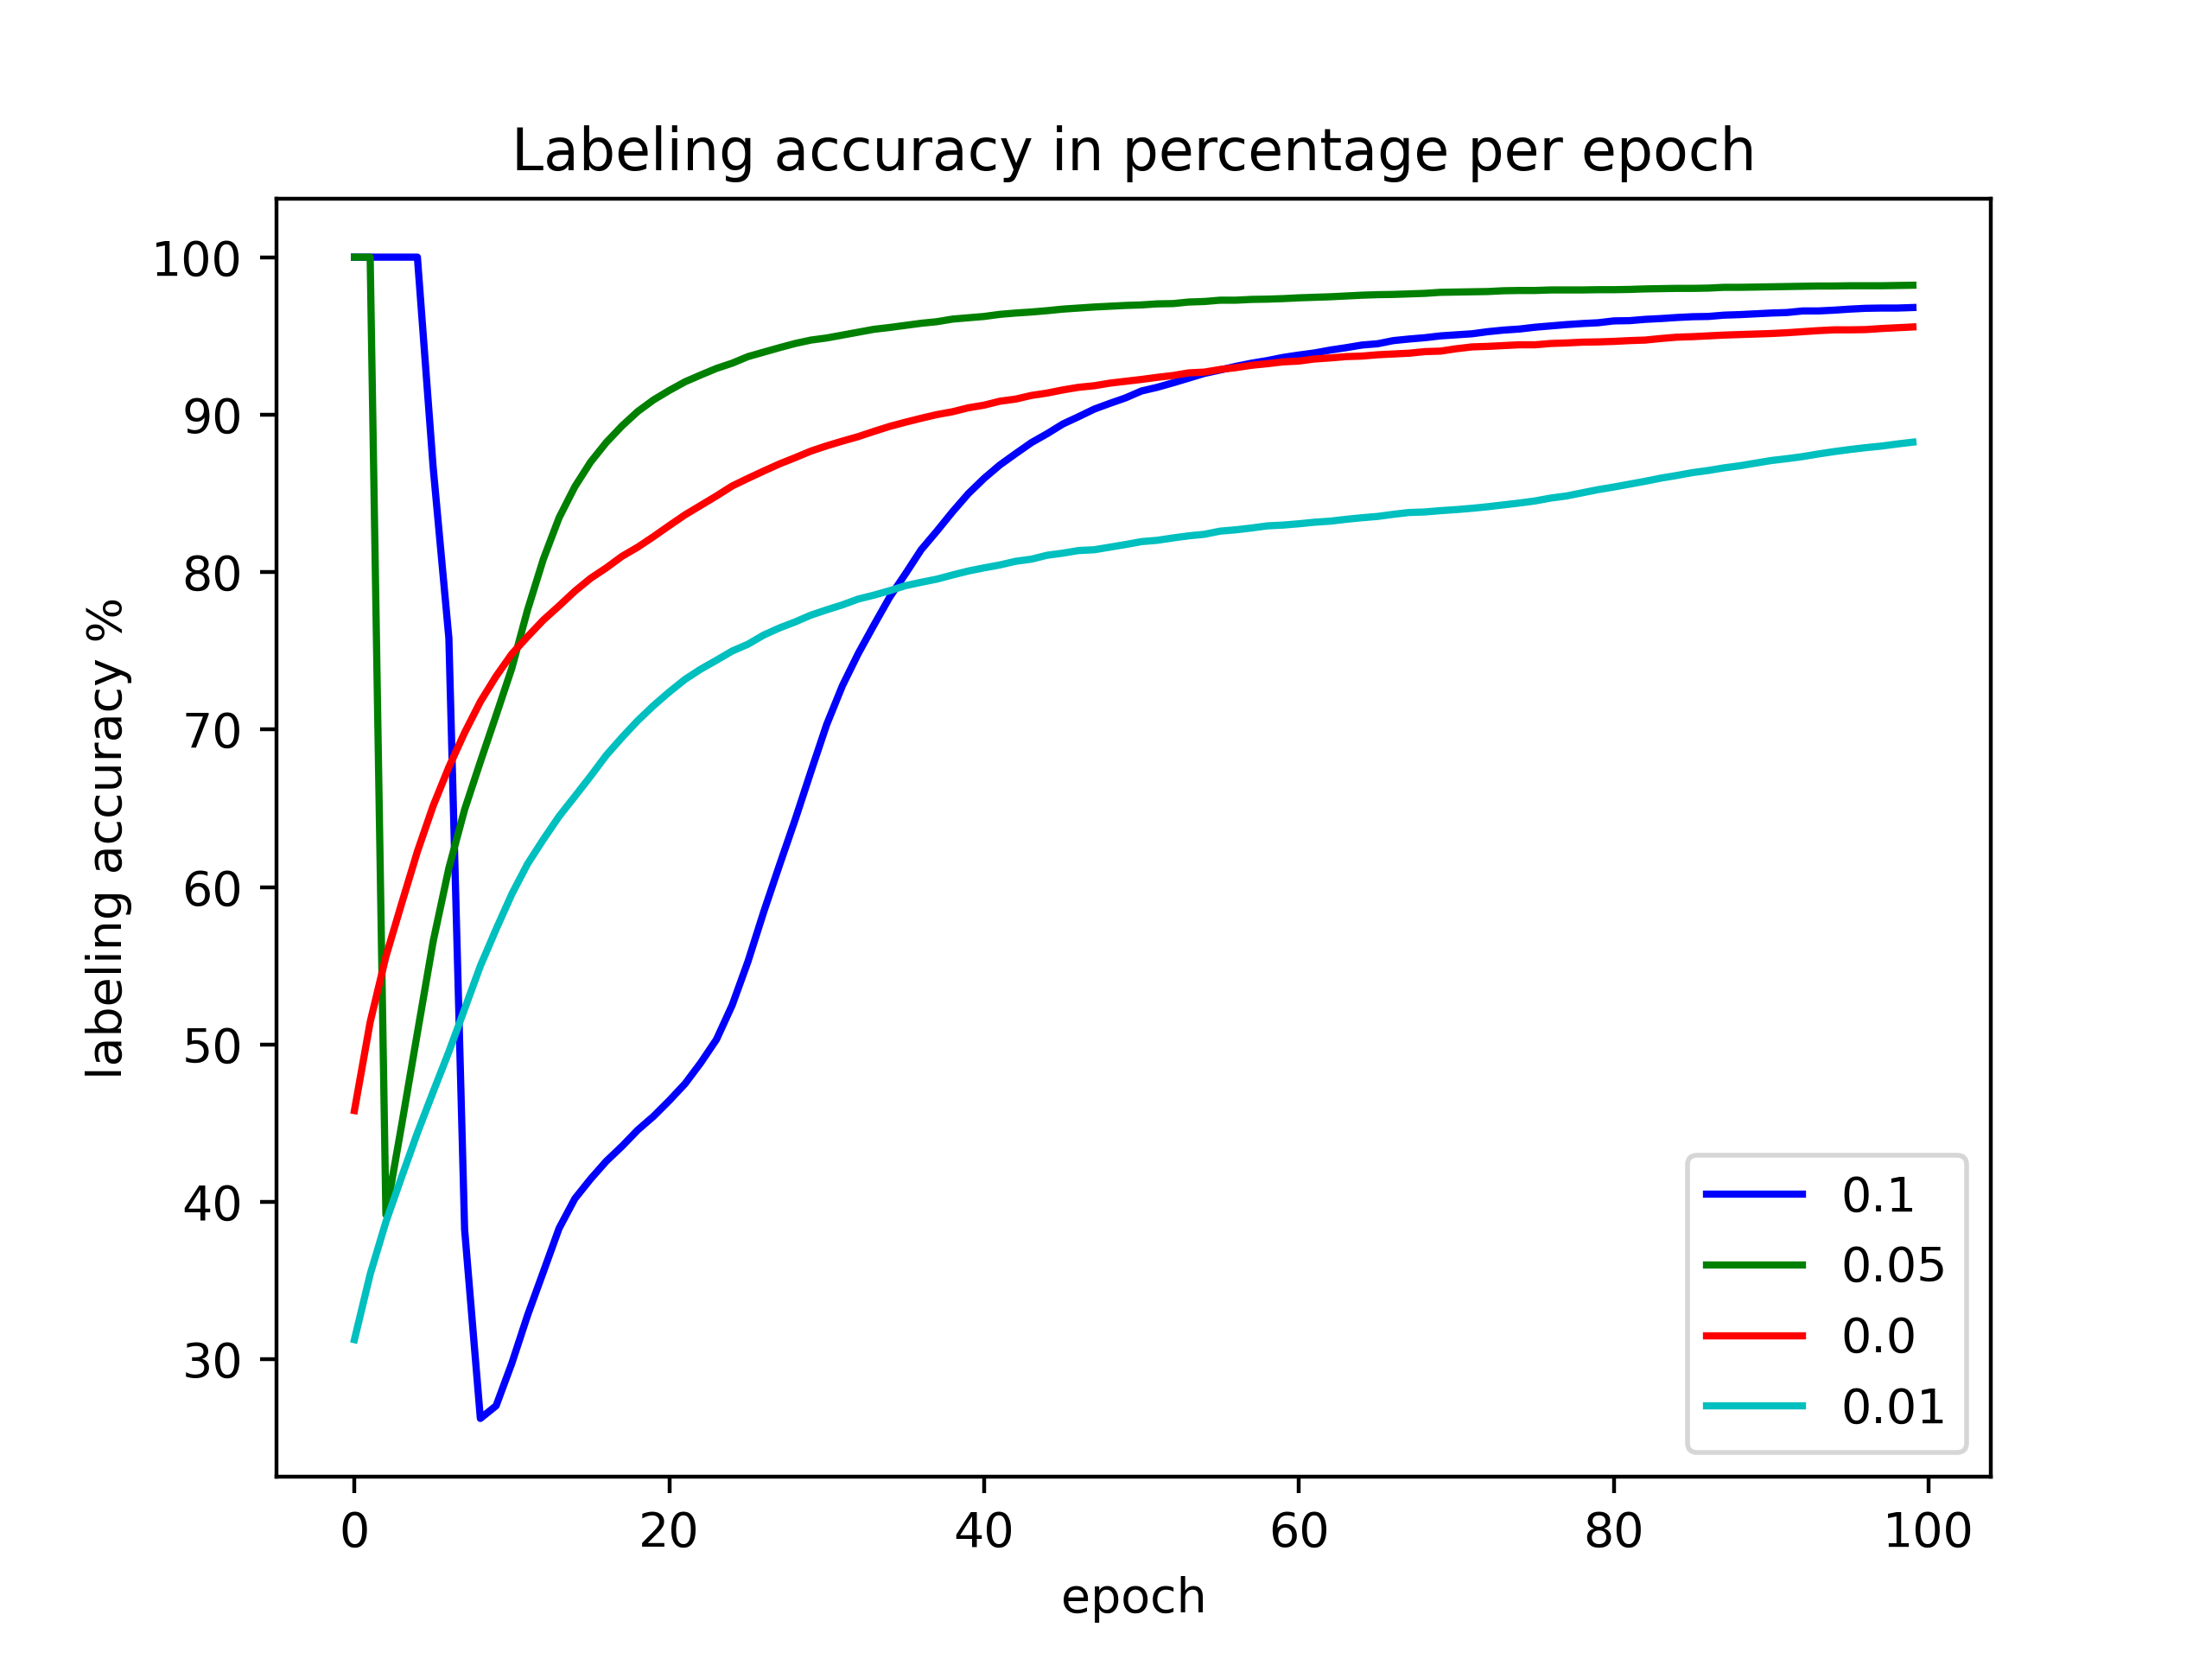
\includegraphics[scale=0.45]{Figures/num_addends_3/labeling_clno.png}} &
\subfloat{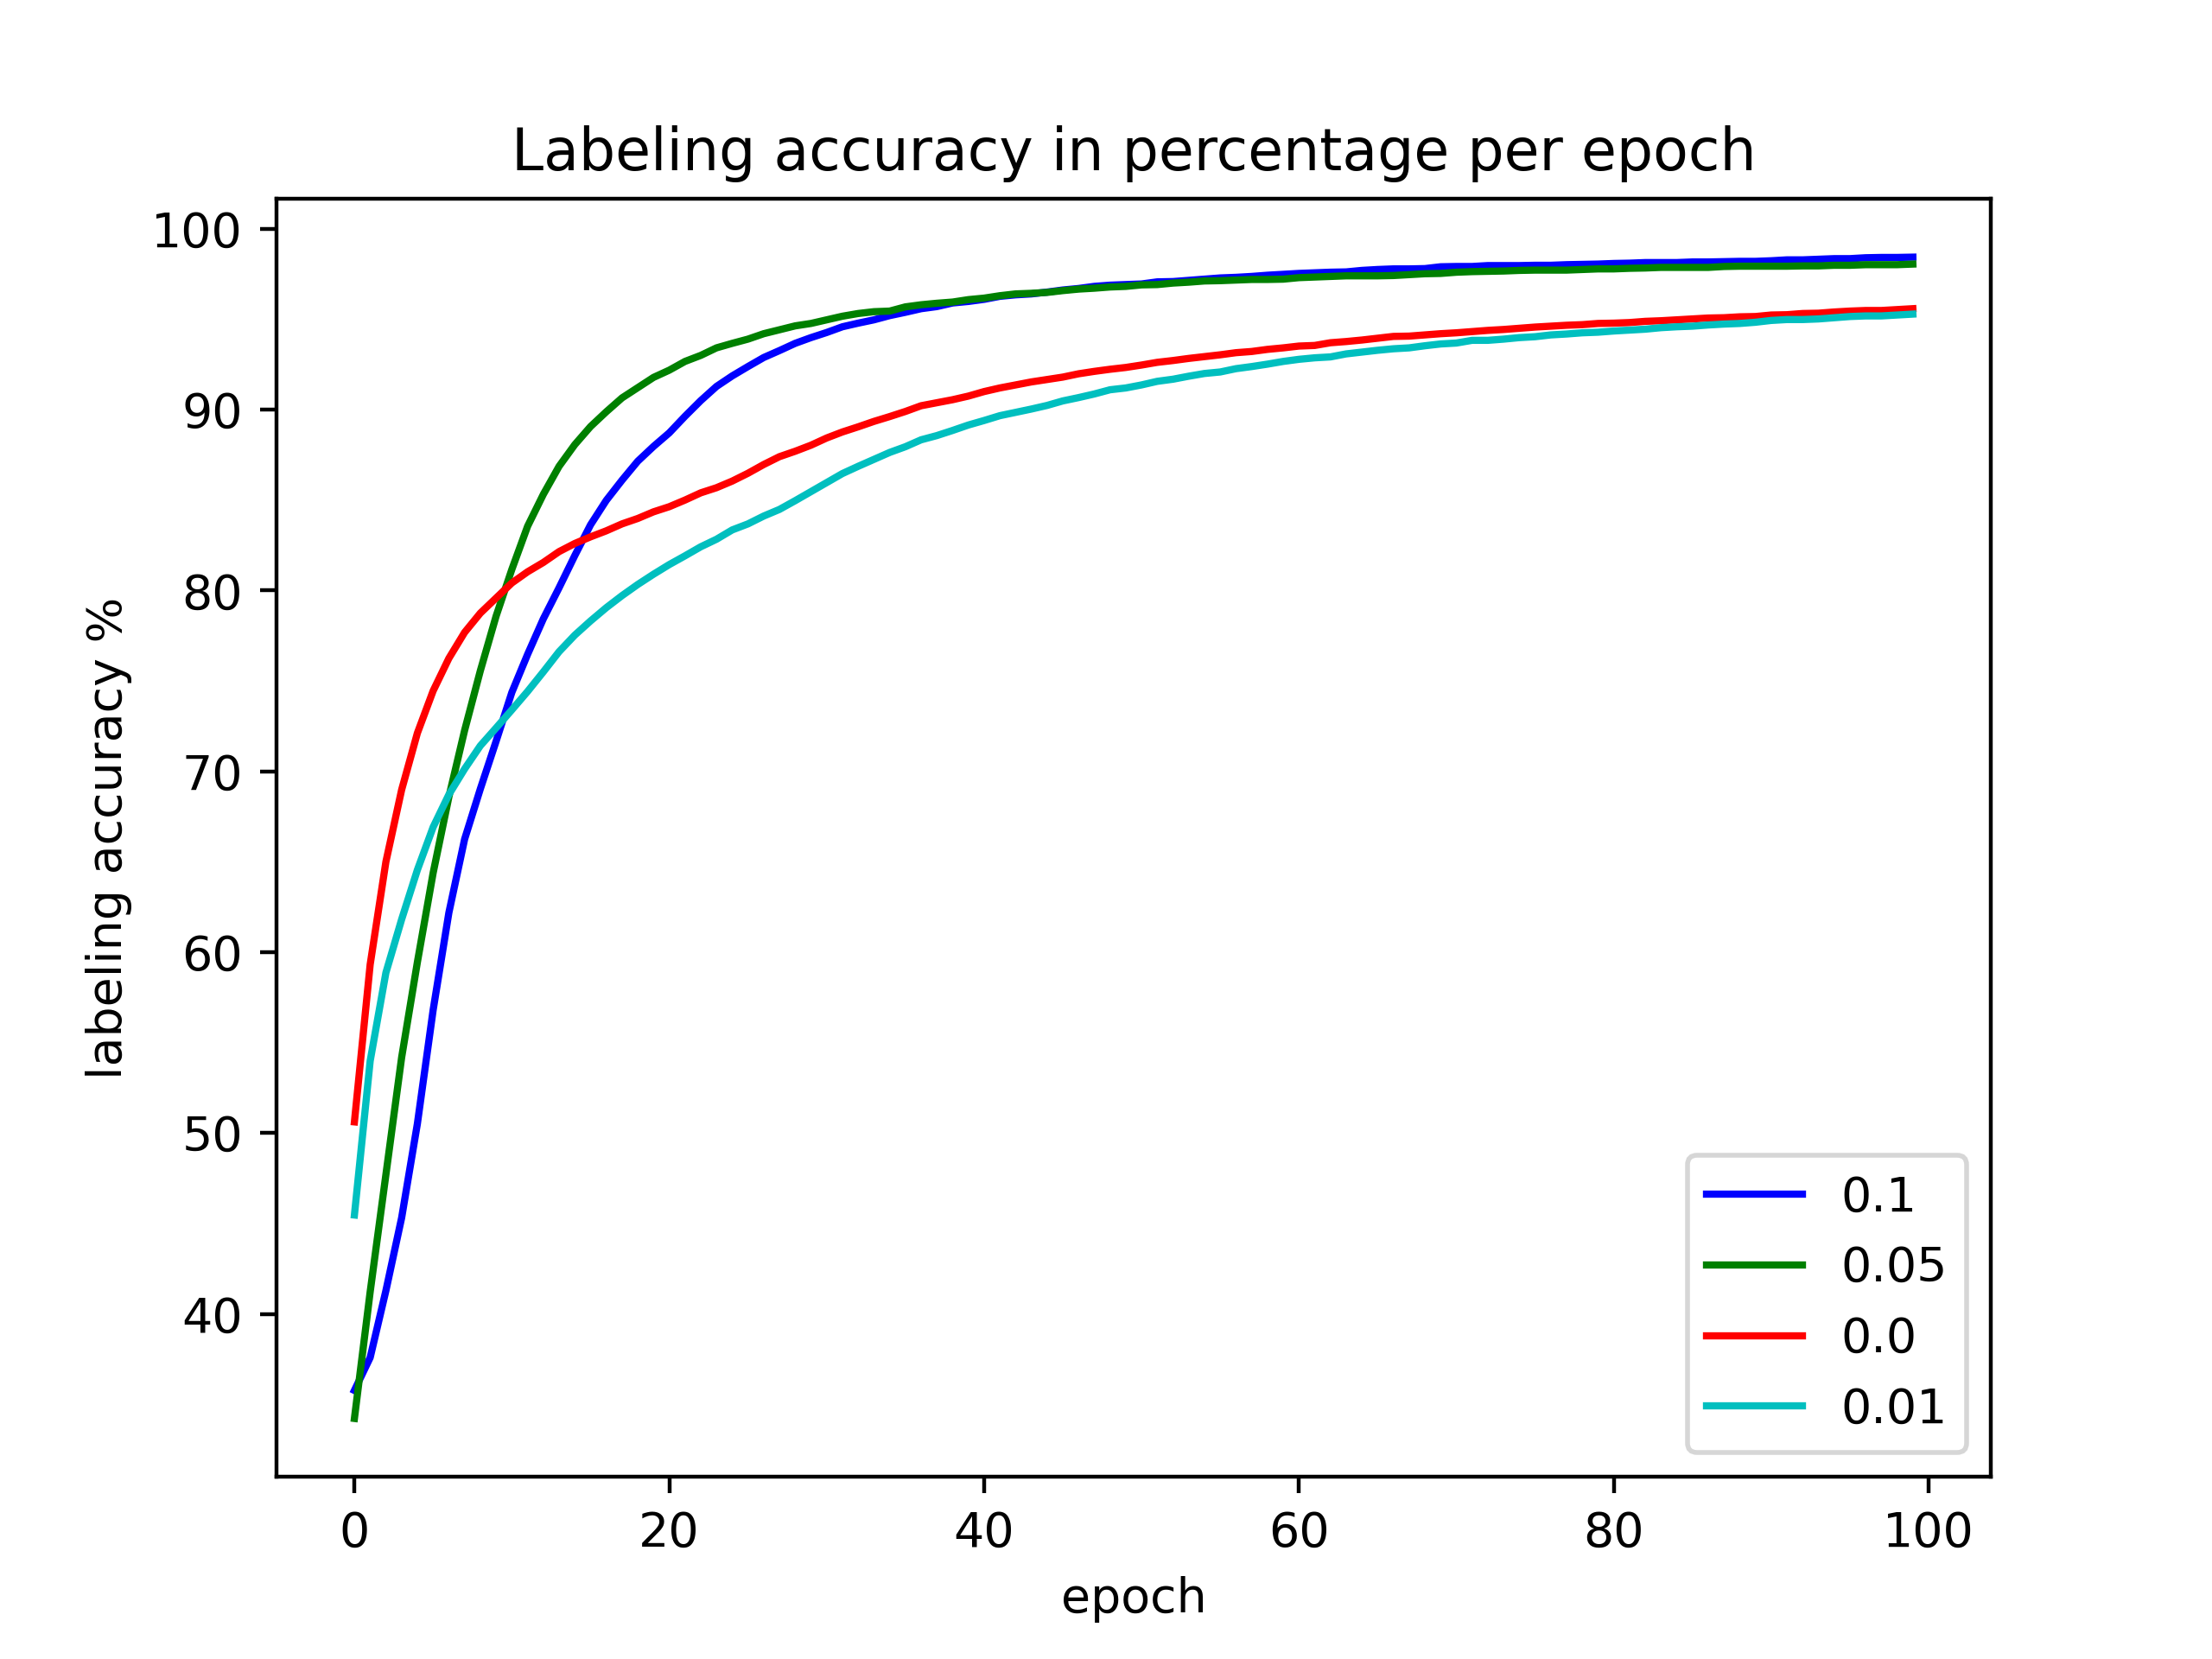
\includegraphics[scale=0.45]{Figures/num_addends_3/labeling_clyes.png}} \\

\subfloat{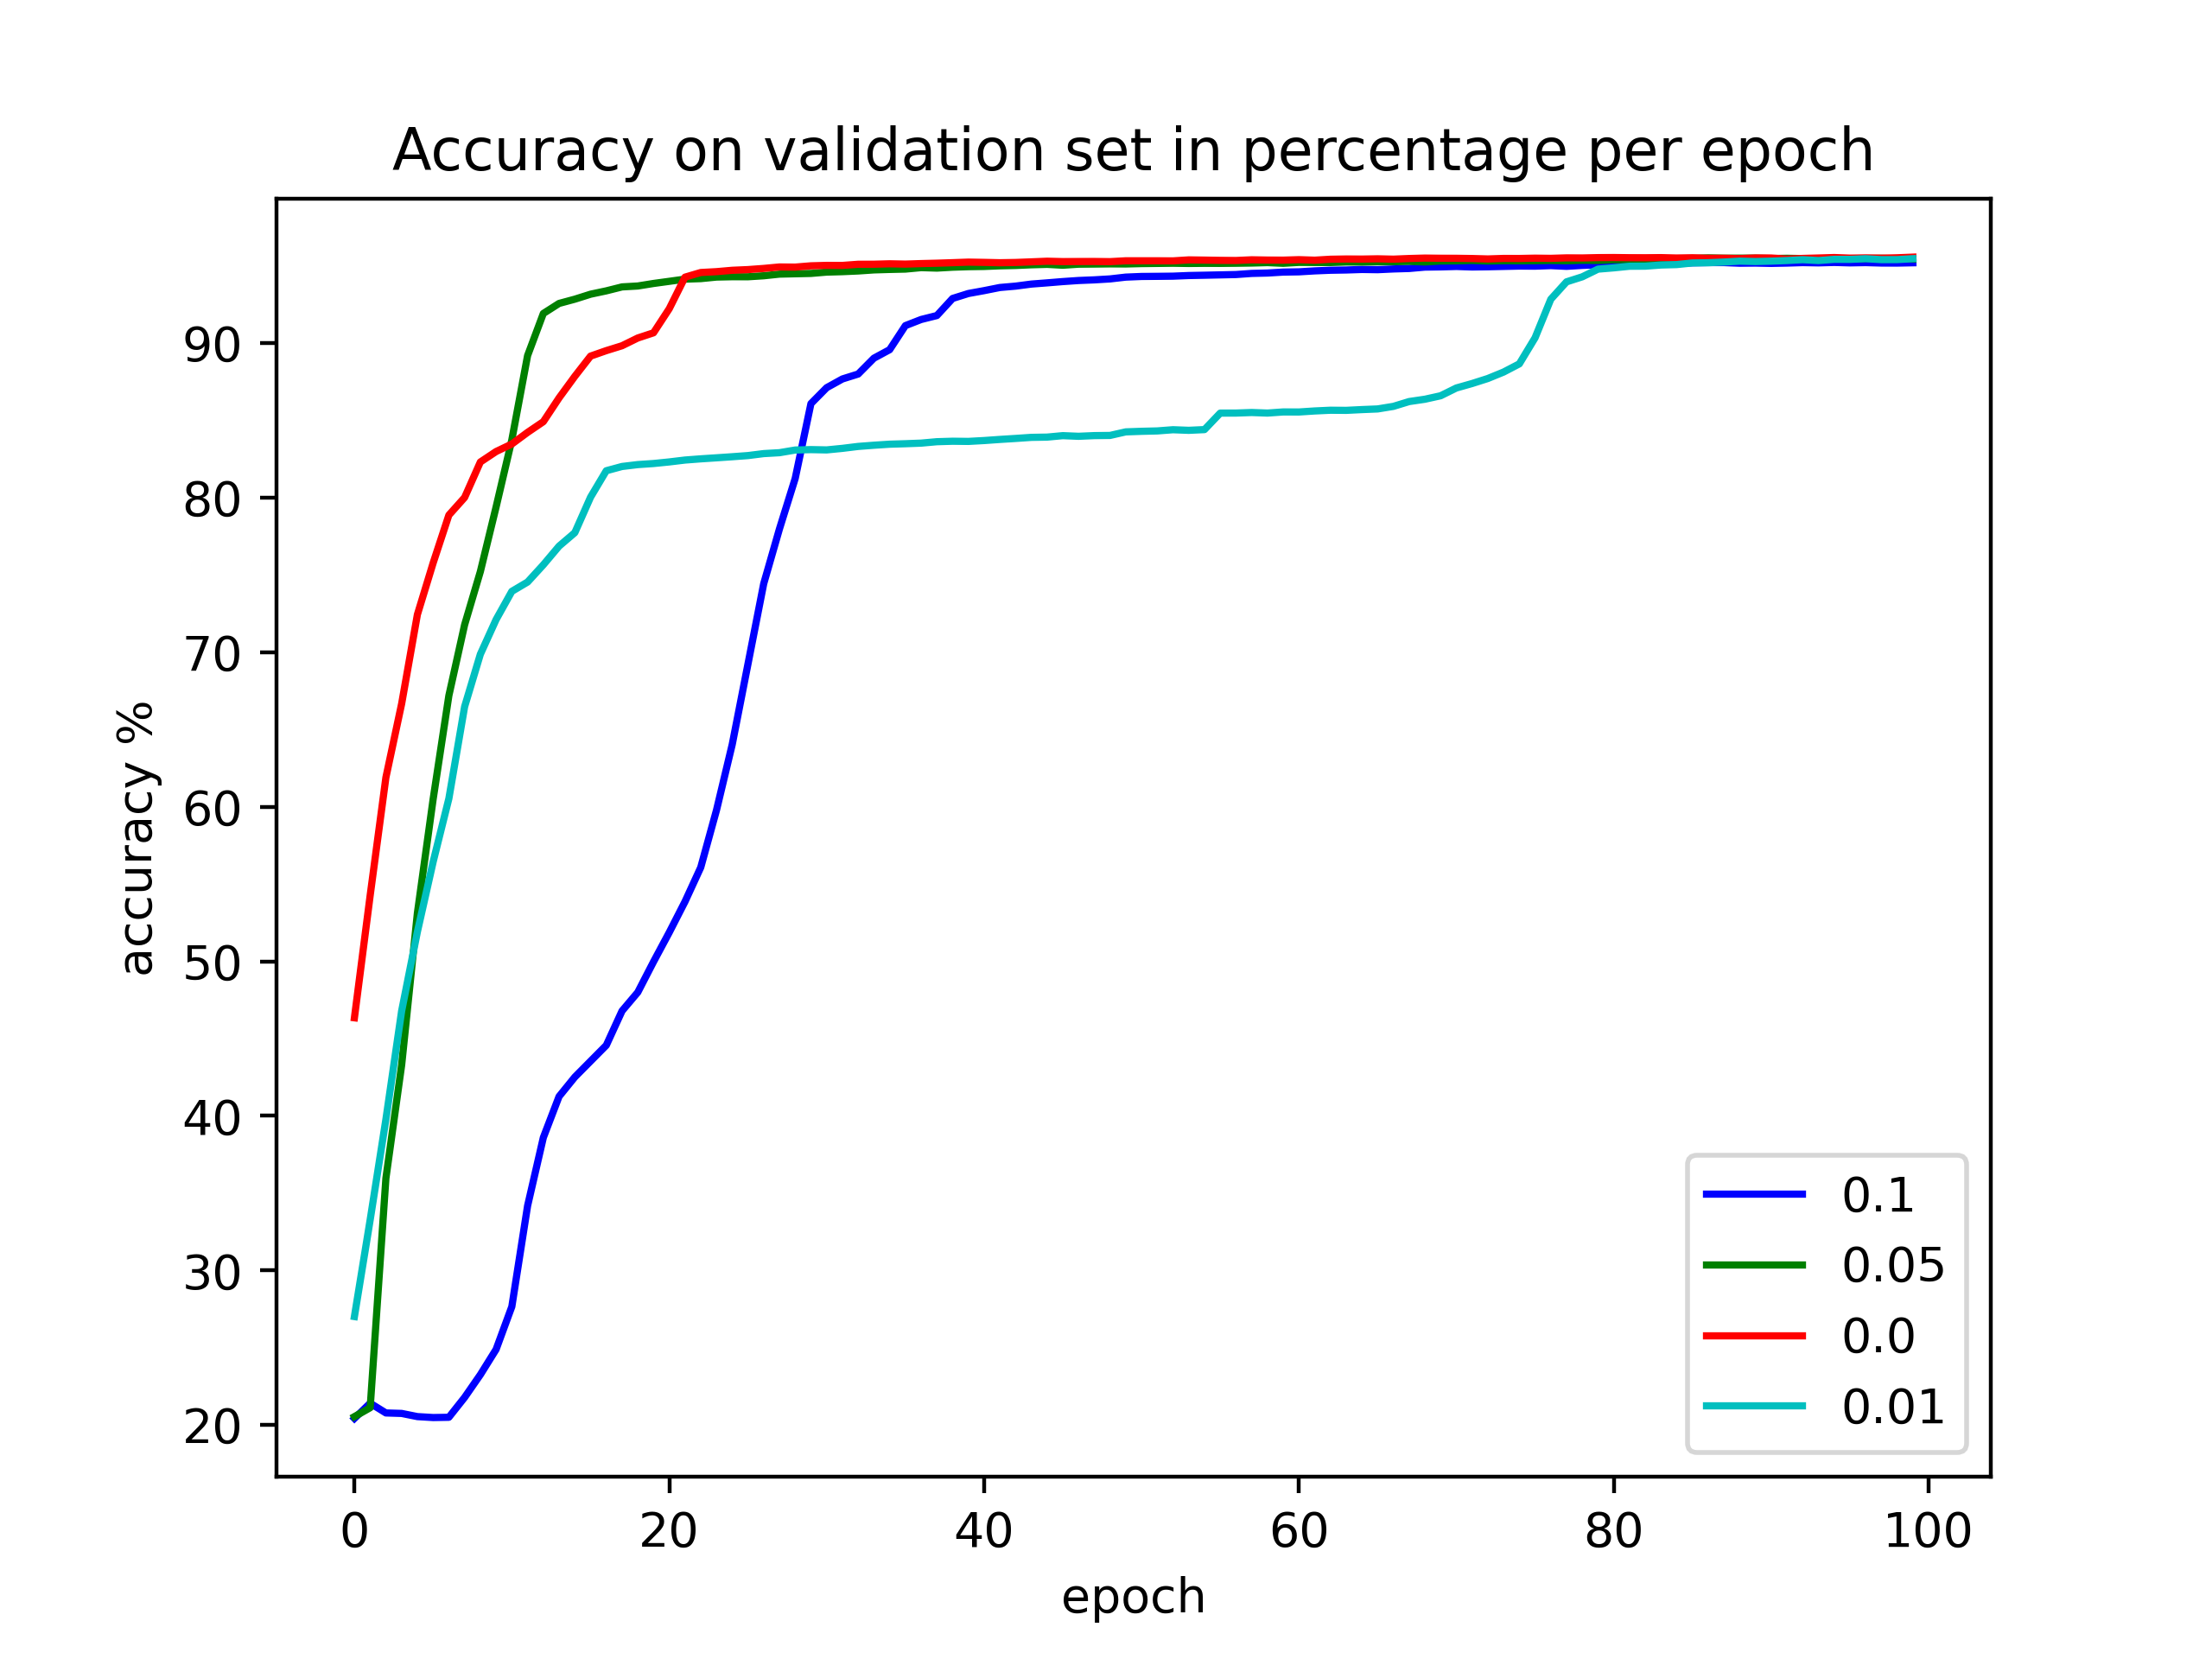
\includegraphics[scale=0.45]{Figures/num_addends_3/accuracy_clno.png}} &
\subfloat{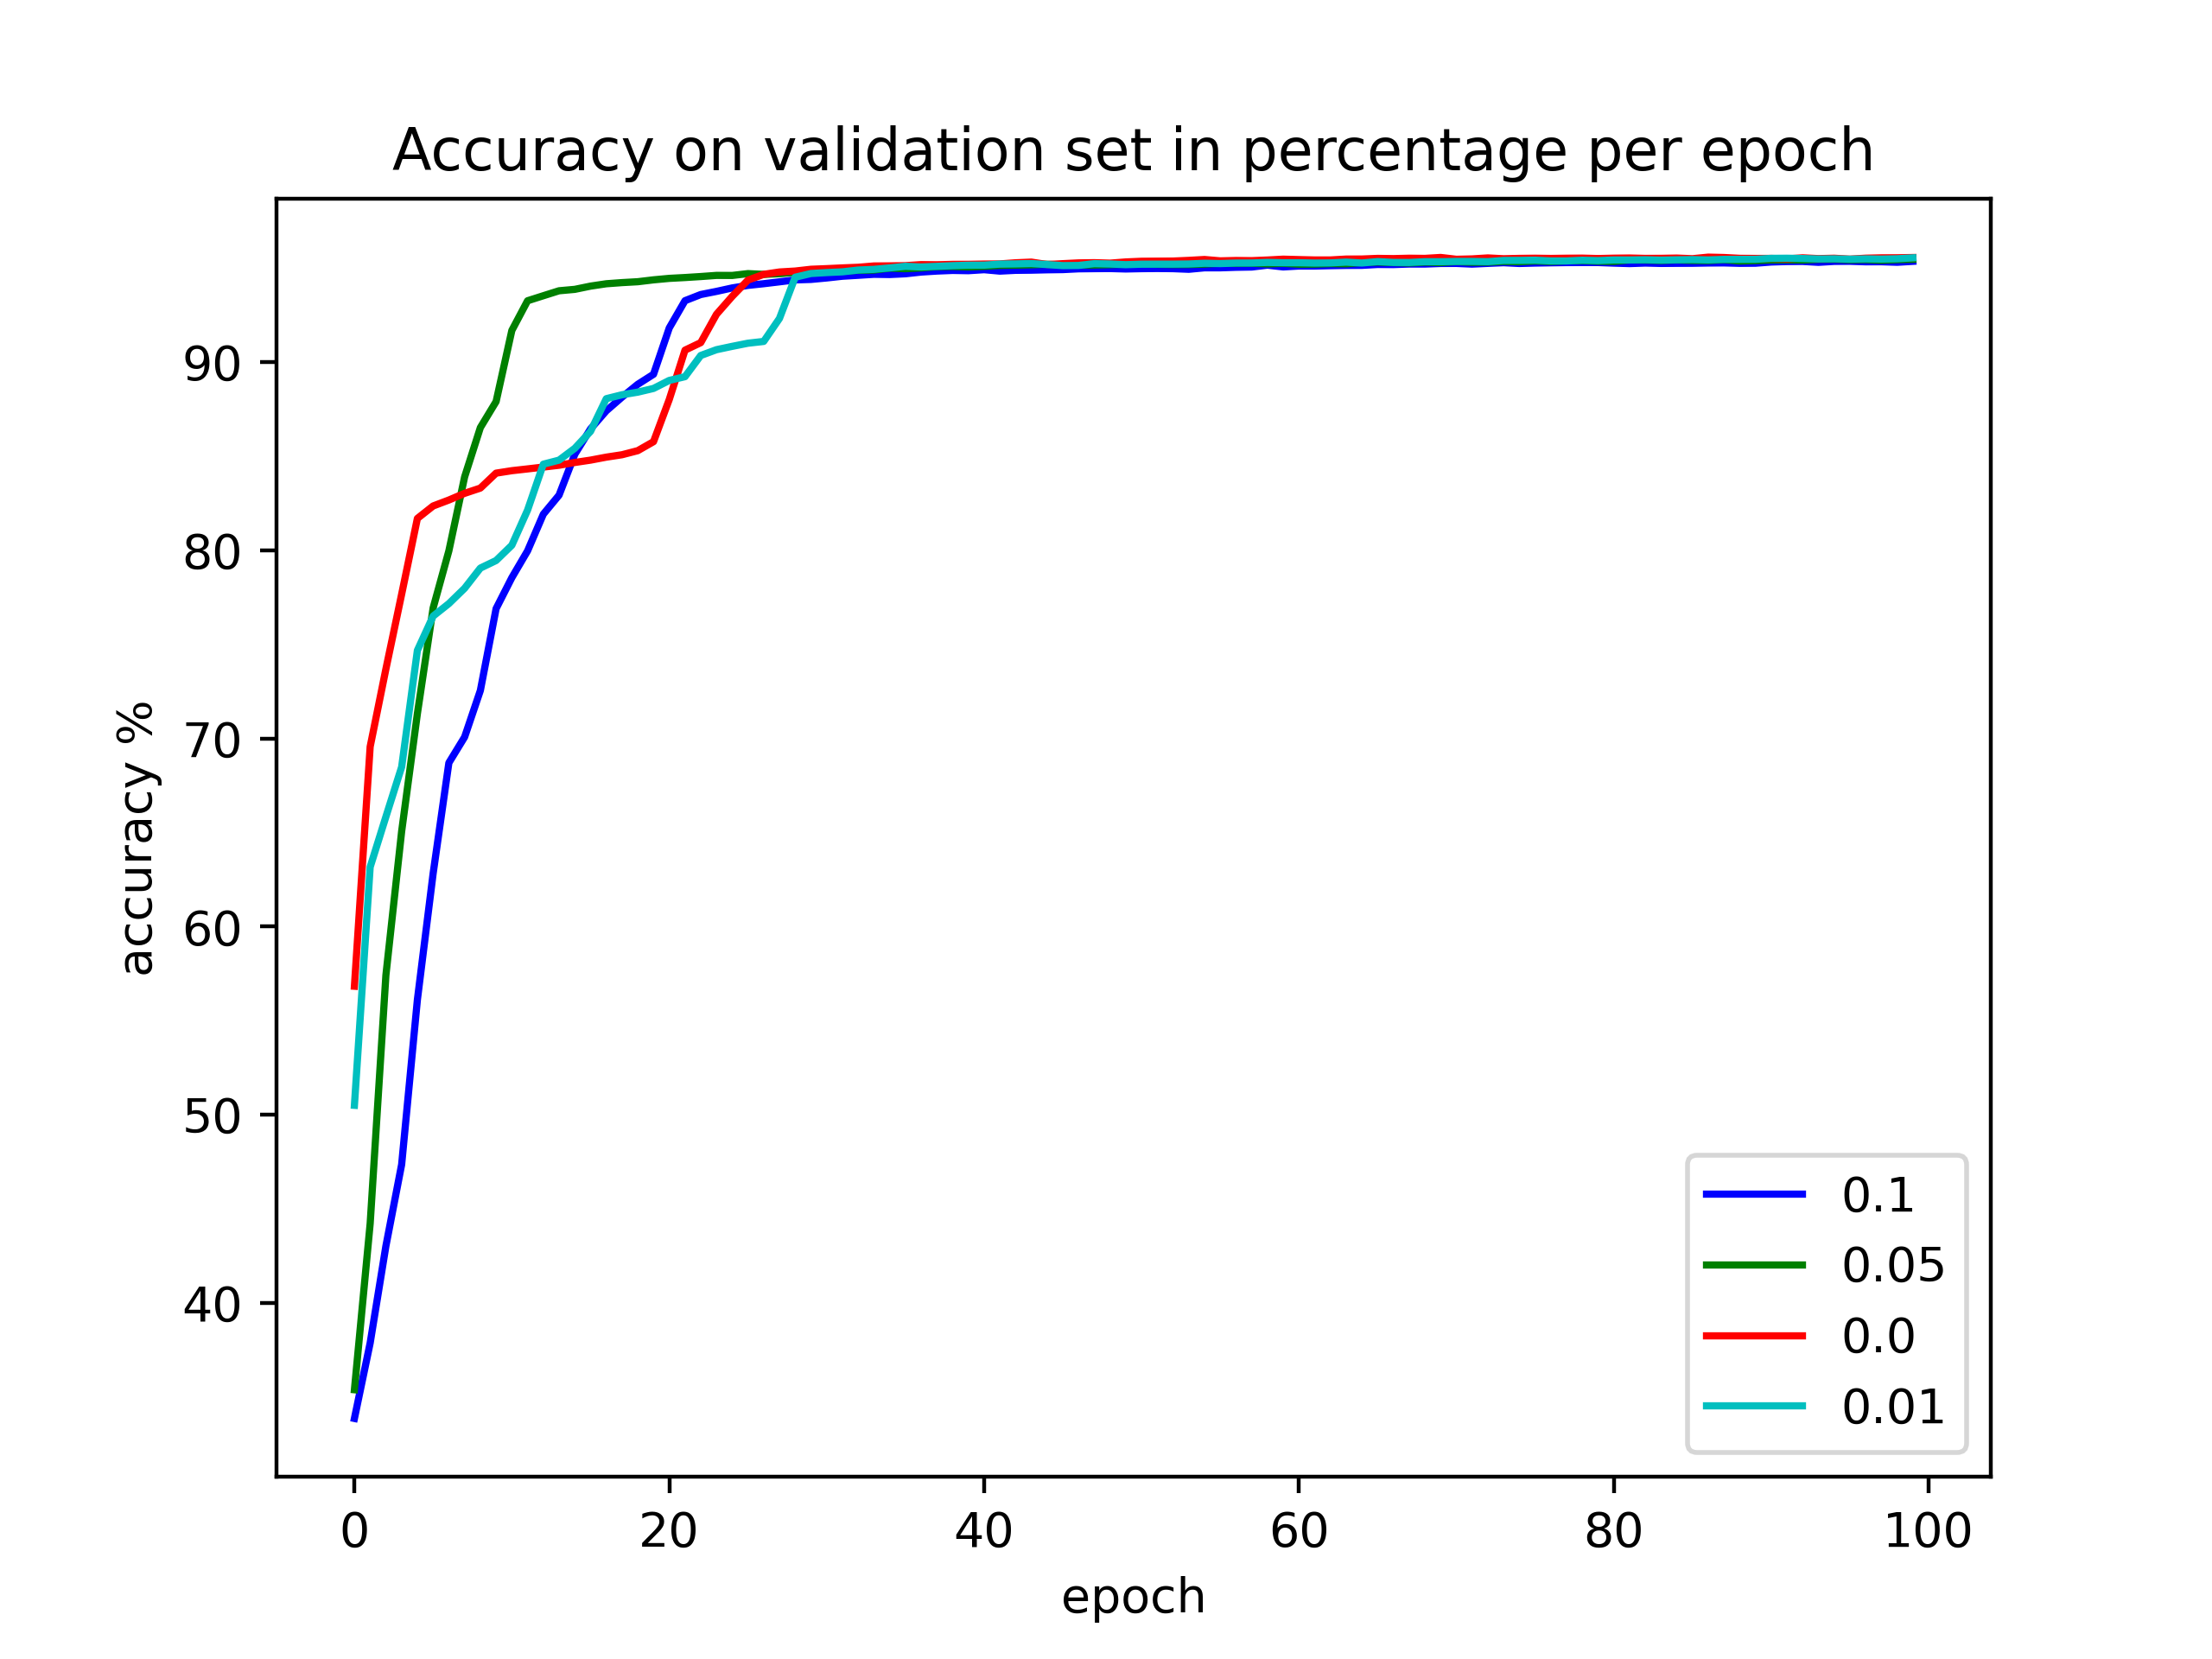
\includegraphics[scale=0.45]{Figures/num_addends_3/accuracy_clyes.png}} \\
\end{longtable}
}
\end{figure}

\subsection{Sum of quadruples}
Table \ref{tab:results-triples-clno} and \ref{tab:results-triples-clyes} show the esperiments results in the case of $m=4$ (i.e., sum of quadruples). We considered the same configurations tested for $m=3$, just slighlty increasing the threshold values. In addition, given the task extreme difficulty (see \ref{tab:info-tasks}), we also explored RAT-SPNs with split depth equal to 2 in the case of enabled pre-training.

\begin{table}[H]
  \centering
  \caption{Performance for $\mathit{f} = sum(\mathit{c}_1,\mathit{c}_2,\mathit{c}_3,\mathit{c}_4)$. Batch size = $100$, number of epochs = $100$, optimization algorithm: \textit{adam}, \textbf{pre-training = false}. All accuracy values are in percentage and approximated to the second digit after the decimal place.}
  \label{tab:results-quadruples-clno}
  \scriptsize
  \begin{tabular}{cccccccrr}
    \toprule
    depth		& distributions 	& splits 		& sums 				& dropout input 		& dropout sums 			& threshold				& valid acc 			& test acc\\
    \midrule
	1	      	& 10     			& 9      		& 10     			& 1     				& 1      				& 0  					& 25.57    				& 26.13\\ 
	1      		& 10     			& 9      		& 10    			& 1      				& 1  					& 0.05    				& 31.30    				& 32.00\\ 
	1	      	& 10     			& 9      		& 10     			& 1      				& 1  					& 0.08    				& 30.85    				& 32.41\\ 
	1   	   	& 10     			& 9      		& 10     			& 1      				& 1  					& 0.11    				& 33.02    				& 34.30\\ 
	1   	   	& 10     			& 9      		& 10 				& 0.75    				& 0.75    				& 0  					& 95.10    				& 95.16\\ 
	1      		& 10     			& 9      		& 10 				& 0.75    				& 0.75    				& 0.05    				& 93.48    				& 93.56\\ 
	1      		& 10     			& 9      		& 10 				& 0.75    				& 0.75    				& 0.08    				& 34.95    				& 35.86\\ 
	1      		& 10     			& 9      		& 10 				& 0.75    				& 0.75    				& 0.11    				& 22.92    				& 23.67\\ 
	
	1      		& 15     			& 14     		& 10     			& 1      				& 1      				& 0  					& 44.37    				& 44.59\\ 
	1      		& 15     			& 14     		& 10     			& 1      				& 1  					& 0.05    				& 25.51    				& 26.02\\ 
	1      		& 15     			& 14     		& 10     			& 1      				& 1  					& 0.08    				& 25.75    				& 26.15\\
	1      		& 15     			& 14     		& 10     			& 1      				& 1  					& 0.11    				& 29.35    				& 30.11\\ 	
	1      		& 15     			& 14     		& 10 				& 0.75    				& 0.75    				& 0						& 22.92    				& 24.03\\ 
	1      		& 15     			& 14     		& 10      			& 0.75    				& 0.75    				& 0.05    				& 25.42    				& 25.40\\ 
	1      		& 15     			& 14     		& 10 				& 0.75    				& 0.75    				& 0.08    				& 30.42    				& 31.32\\ 
	1      		& 15     			& 14     		& 10 				& 0.75    				& 0.75    				& 0.11					& 21.32    				& 21.94\\
	
	1  			& 20     			& 19			& 10				& 1						& 1      				& 0			      		& 36.21 				& 36.78\\ 
	1      		& 20     			& 19     		& 10     			& 1      				& 1      				& 0.01    				& 28.15    				& 28.99\\ 
	1      		& 20     			& 19     		& 10     			& 1      				& 1      				& 0.05    				& 35.68    				& 36.73\\
	1      		& 20     			& 19     		& 10     			& 1      				& 1      				& 0.10    				& 41.23    				& 43.58\\
	1      		& 20     			& 19     		& 10     			& 0.75      			& 0.75      			& 0	    				& 26.18    				& 26.89\\
	1      		& 20     			& 19     		& 10     			& 0.75      			& 0.75      			& 0.01    				& 93.12    				& 93.26\\
	1      		& 20     			& 19     		& 10     			& 0.75      			& 0.75      			& 0.05    				& 23.88    				& 24.00\\
	1      		& 20     			& 19     		& 10     			& 0.75      			& 0.75      			& 0.10    				& 34.11    				& 35.79\\ 
    \bottomrule
  \end{tabular}
\end{table}

\begin{table}[H]
  \centering
  \caption{Performance for $\mathit{f} = sum(\mathit{c}_1,\mathit{c}_2,\mathit{c}_3,\mathit{c}_4)$. Batch size = $100$, number of epochs = $100$, optimization algorithm: \textit{adam}, \textbf{pre-training = true}. All accuracy values are in percentage and approximated to the second digit after the decimal place.}
  \label{tab:results-quadruples-clyes}
  \scriptsize
  \begin{tabular}{cccccccrr}
    \toprule
    depth		& distributions 	& splits 		& sums 				& dropout input 		& dropout sums 			& threshold				& valid acc 			& test acc\\
    \midrule
	1 			& 10     			& 9 			& 10     			& 1 					& 1 					& 0 					& 43.92   				& 44.67\\
	1 			& 10     			& 9 			& 10     			& 1 					& 1 					& 0.05    				& 30.05    				& 31.48\\
	1 			& 10     			& 9 			& 10     			& 1 					& 1 					& 0.08    				& 28.80    				& 28.62\\
	1 			& 10     			& 9 			& 10     			& 1 					& 1 					& 0.11    				& 26.63    				& 26.67\\
	1 			& 10     			& 9 			& 10     			& 0.75    				& 0.75    				& 0 					& 96.55    				& 96.10\\
	1 			& 10     			& 9 			& 10     			& 0.75    				& 0.75    				& 0.05    				& 96.23    				& 95.79\\
	1 			& 10     			& 9 			& 10     			& 0.75    				& 0.75    				& 0.08    				& 34.78    				& 34.94\\
	1 			& 10     			& 9 			& 10     			& 0.75    				& 0.75    				& 0.11   				& 32.07    				& 31.75\\
	
	1 			& 15     			& 14     		& 10     			& 1 					& 1 					& 0 					& 94.83    				& 94.43\\
	1 			& 15     			& 14     		& 10     			& 1 					& 1 					& 0.05   				& 24.83    				& 25.73\\
	1 			& 15     			& 14     		& 10     			& 1 					& 1 					& 0.08    				& 34.62    				& 35.90\\
	1 			& 15     			& 14     		& 10     			& 1 					& 1 					& 0.11    				& 35.38    				& 35.71\\
	1 			& 15     			& 14     		& 10     			& 0.75    				& 0.75    				& 0 					& 96.05    				& 96.07\\	
	1 			& 15     			& 14     		& 10     			& 0.75    				& 0.75    				& 0.05    				& 96.35    				& 96.17\\
	1 			& 15     			& 14     		& 10     			& 0.75    				& 0.75    				& 0.08    				& 32.92    				& 33.92\\
	1 			& 15     			& 14     		& 10     			& 0.75    				& 0.75    				& 0.11   				& 27.30    				& 28.35\\

	1  			& 20     			& 19			& 10				& 1						& 1      				& 0			      		& 93.00 				& 94.12\\ 
	1      		& 20     			& 19     		& 10     			& 1      				& 1      				& 0.01    				& 31.65    				& 32.78\\ 
	1      		& 20     			& 19     		& 10     			& 1      				& 1      				& 0.05    				& 25.89    				& 26.37\\
	1      		& 20     			& 19     		& 10     			& 1      				& 1      				& 0.10    				& 44.20    				& 45.99\\
	1      		& 20     			& 19     		& 10     			& 0.75      			& 0.75      			& 0	    				& 31.54    				& 33.42\\
	1      		& 20     			& 19     		& 10     			& 0.75      			& 0.75      			& 0.01    				& 94.11    				& 95.56\\
	1      		& 20     			& 19     		& 10     			& 0.75      			& 0.75      			& 0.05    				& 28.23    				& 28.35\\
	1      		& 20     			& 19     		& 10     			& 0.75      			& 0.75      			& 0.10    				& 33.51    				& 33.93\\
	
	
	2 			& 10     			& 8 			& 10     			& 1 					& 1 					& 0 					& 19.92    				& 20.35\\
	2 			& 10     			& 8 			& 10     			& 1 					& 1 					& 0.05   				& 24.18    				& 25.09\\
	2 			& 10     			& 8 			& 10     			& 1 					& 1 					& 0.08    				& 32.20    				& 33.14\\
	2 			& 10     			& 8 			& 10     			& 1 					& 1 					& 0.11    				& 37.87    				& 37.39\\	
	2 			& 10     			& 8 			& 10     			& 0.75    				& 0.75    				& 0 					& 97.60    				& 97.15\\
	2 			& 10     			& 8 			& 10     			& 0.75    				& 0.75    				& 0.05    				& 33.80    				& 33.48\\
	2 			& 10     			& 8 			& 10     			& 0.75    				& 0.75    				& 0.08    				& 36.53    				& 36.09\\
	2 			& 10     			& 8 			& 10     			& 0.75    				& 0.75    				& 0.11    				& 37.98    				& 38.01\\

	2 			& 15     			& 12     		& 15     			& 1 					& 1 					& 0 					& 20.73    				& 21.00\\
	2 			& 15     			& 12     		& 15     			& 1 					& 1 					& 0.05    				& 25.07    				& 25.58\\
	2 			& 15     			& 12     		& 15     			& 1 					& 1 					& 0.08    				& 33.50    				& 34.02\\
	2 			& 15     			& 12     		& 15     			& 1 					& 1 					& 0.11    				& 39.42    				& 40.47\\
	2 			& 15     			& 12     		& 15     			& 0.75    				& 0.75    				& 0 					& 26.00    	 			& 26.81\\
	2 			& 15     			& 12     		& 15     			& 0.75    				& 0.75    				& 0.08    				& 37.48    				& 38.26\\
	2 			& 15     			& 12     		& 15     			& 0.75    				& 0.75    				& 0.05    				& 27.82    				& 28.84\\
	2 			& 15     			& 12     		& 15     			& 0.75    				& 0.75    				& 0.11    				& 41.52    				& 42.50\\
    \bottomrule
  \end{tabular}
\end{table}
Unfortunately, the behaviour shown by the above tables is similar to the one highlighted in Table \ref{tab:simple-model}: performance varies greatly from one configuration to another, indicating that the lerning is no longer deterministic, but prone to chance. Nevertheless, with respect to Table \ref{tab:simple-model}, we note a significant difference: there are no "intermediate" accuracy values, basically the model converges or doesn't learn at all. This could mean that, if the model "finds the correct direction", it is always able to converge and achieve good performance.

Given the non-deterministic nature of learning, in this case it is not interesting to evaluate the model behaviour as in Figures \ref{fig:thresholds-triples}. Nevertheless, we want to understand if the pre-training can still bring some advantages. For this purpose, Table \ref{tab:comparison-pre-training} compares corresponding configurations (with depth equal to 1) of the pre-trained model and the not pre-trained one, taking into account \textit{(i)} the number of considered examples and \textit{(ii)} the ratios of examples labeling accuracy of digit from 0 to 2. The analysis is limited to the first epoch, because it is the most influenced by the pre-training, and to such digits, because we observed that the pre-training perform only on \textit{zero} examples (for this specific task). Results highlighted by such analysis are evident: the examples labeling accuracy is always higher when the pre-training is enabled, except for two not relevant cases in which it is slighlty lower, but in the face of a greater number of considered examples.

We can conclude that the pre-training still correctly works, but it is no longer sufficient, in conjunction with the abduction threshold, to solve such a difficult task. 

\begin{table}[H]
  \centering
  \caption{Comparison between corresponding configurations (with split depth = 1) of the pre-trained model and the not pre-trained one, with reference to Tables \ref{tab:results-quadruples-clno} and \ref{tab:results-quadruples-clyes}. \#(examples) refers to the number of considered examples during the current training epoch, while $R_i$ refers to the ratio of examples labeling accuracy of the \textit{i-th} digit. All the reported values refer to the \textbf{first} training epoch. Greater $R_i$ values between corresponding configurations are highlighted in bold.}
  \label{tab:comparison-pre-training}
  \small
  \begin{tabular}{cccc|cccc}
	\multicolumn{4}{c|}{\textbf{Pre-training = true}} & \multicolumn{4}{c}{\textbf{Pre-training = false}}\\
	\hline
	\multicolumn{1}{c}{\#(examples)} & $R_0$ & $R_1$ & $R_2$ & 
	\multicolumn{1}{c}{\#(examples)} & $R_0$ & $R_1$ & \multicolumn{1}{c}{$R_2$} \\
	\hline
	54000	& \textbf{0.90}	& \textbf{0.89}	& \textbf{0.06}	& 54000	& 0.64	& 0.02	& 0.05 \\
	32		& 0.95	& 0.33	& -		& 12	& \textbf{1}	& -		& - \\
	12		& 1		& -		& -		& 12	& 1		& -		& - \\
	12		& 1		& -		& -		& 12	& 1		& -		& - \\
	54000	& \textbf{0.93}	& \textbf{0.86}	& \textbf{0.14}	& 54000	& 0.83	& 0.05	& 0.08 \\
	36		& 1		& \textbf{1}		& -	& 12	& 1		& -		& - \\
	12		& 1		& -		& -		& 12	& 1		& -		& - \\
	12		& 1		& -		& -		& 12	& 1		& -		& - \\
	
	54000	& \textbf{0.90}	& \textbf{0.81}	& \textbf{0.13}	& 54000 & 0.89	& 0.14	& 0.08 \\
	52		& 1		& 0.33	& 0.67	& 12	& 1		& -		& - \\
	12		& 1		& -		& -		& 12	& 1		& -		& - \\
	12		& 1		& -		& -		& 12	& 1		& -		& - \\
	54000	& \textbf{0.89}	& \textbf{0.94}	& \textbf{0.31}	& 54000 & 0.88	& 0.85	& 0.06 \\
	12		& 1		& -		& -		& 12	& 1		& -		& - \\
	12		& 1		& -		& -		& 12	& 1		& -		& - \\
	12		& 1		& -		& -		& 12	& 1		& -		& - \\
	
	54000	& \textbf{0.91}	& \textbf{0.88}	& \textbf{0.12}	& 54000	& 0.60	& 0.06	& 0.02 \\
	40		& 0.97	& 0.41	& -		& 12	& \textbf{1}	& -		& - \\
	12		& 1		& -		& -		& 12	& 1		& -		& - \\
	12		& 1		& -		& -		& 12	& 1		& -		& - \\
	54000	& \textbf{0.92}	& \textbf{0.85}	& \textbf{0.12}	& 54000	& 0.79	& 0.25	& 0.04 \\
	12		& 1		& -		& -		& 12	& 1		& -		& - \\
	12		& 1		& -		& -		& 12	& 1		& -		& - \\
	12		& 1		& -		& -		& 12	& 1		& -		& - \\
   \end{tabular}
\end{table}
\chapter{Conclusions and Future Work}
\label{ChapterConclusions} 
Neural-symbolic computing aims at integrating two most fundamental cognitive abilities: the ability to learn from the environment, and the ability to reason from what has been learned. Neural-symbolic computing has been an active topic of research for many years, reconciling the advantages of robust learning in neural networks and reasoning and interpretability of symbolic representation.

In this thesis, we explored the integration between \textit{Sum-Product networks} (specifically \textit{Random-And-Tensorized SPNs}) and \textit{abductive reasoning}, applied to a more difficult classification task, in which the known information about training examples is not directly their associated class but an aggregate information deriving from it. We stressed the model robustness by increasing the task difficulty, that is increasing the number of possible abductions and decreasing the number of certainties (i.e., observations for which just one possible label can be abduced). Experiments results showed that both the implemented solutions and \textit{RAT-SPNs} have proved to be adequate (but not always sufficient) in dealing with a task of this kind.

In the following, we outline some possible future works:

\begin{itemize}
	\item to explore the model behaviour with SPNs having higher split depths, in order to understand if the use of more complex models might bring some advantages;
	\item to deal with tasks in which the number of possible abductions for some observations is so high that it requires a pruning mechanism. Such cases would need to increase the interaction between symbolic and sub-symbolic modules, specifically during the training phase;
	\item to implement an \textit{adaptive} abduction threshold, that varies according to the learning model degree within both the same training epoch and different ones;
	\item to use a loss function that penalizes errors in a manner directly proportional to the probability of the corresponding abduction;
	\item to ensure in some way a consistency in examples labeling by the model.
\end{itemize}

 


%----------------------------------------------------------------------------------------
%	BIBLIOGRAPHY
%----------------------------------------------------------------------------------------

%\raggedright
\printbibliography[heading=bibintoc]
\nocite{*}

%----------------------------------------------------------------------------------------

\end{document}  
